%%% File encoding: UTF-8
%%% äöüÄÖÜß  <-- no German umlauts here? Use an UTF-8 compatible editor!

%%% Magic comments for setting the correct parameters in compatible IDEs
% !TeX encoding = utf8
% !TeX program = pdflatex 
% !TeX spellcheck = de_DE
% !BIB program = biber

\documentclass[bachelor,english,smartquotes]{hgbthesis}
% Valid options in [..]: 
%    Type of work: 'diploma', 'master' (default), 'bachelor', 'internqship' 
%		 Additionally for a thesis exposé: 'proposal (for 'bachelor' and 'master')
%    Main language: 'german' (default), 'english'
%    Turn on smart quote handling: 'smartquotes'
%    APA bibliography style: 'apa'
%%%-----------------------------------------------------------------------------

\RequirePackage[utf8]{inputenc} % Remove when using lualatex or xelatex!

% add. package commands
\usepackage{forest}

\logofile{logo}           % Logo file: images/logo.pdf (no logo: \logofile{})
\bibliography{references} % Biblatex bibliography file (references.bib)

%%%-----------------------------------------------------------------------------
\begin{document}
%%%-----------------------------------------------------------------------------

%%%-----------------------------------------------------------------------------
% Title page entries
%%%-----------------------------------------------------------------------------

\title{Theorema Project: Document Processing \\
    \large Entwurfsversion vom \today \\ 
    (mit alternativem Deckblatt)}
\author{Jack C. Heseltine, BA}
\programname{Software Engineering}

\programtype{Fachhochschul-Bachelorstudiengang} % select/edit
%\programtype{Fachhochschul-Masterstudiengang}

\placeofstudy{Hagenberg, Fachhochschule Oberösterreich, in Kooperation mit RISC, \\
    dem Research Institute Symbolic Computation (Johannes Kepler Universität Linz) \\
    zur Erlangung des akademischen Grades \\ % should also be included
    Bachelor of Science in Engineering}
\dateofsubmission{2024}{09}{30} % {YYYY}{MM}{DD}

\advisor{Assoc. Univ.-Prof. DI Dr. Wolfgang Windsteiger} % optional

%\strictlicense % restrictive license instead of Creative Commons (discouraged!)

%%%-----------------------------------------------------------------------------
\frontmatter                                   % Front part (roman page numbers)
%%%-----------------------------------------------------------------------------

\maketitle
\tableofcontents

\chapter{Preface}

[[Thank Red Cross/Blood Bank, for enabling bb studies? To bring them preprint when I visit.]]



 % A preface is optional
\chapter{Abstract}

This work explores the Wolfram Language as a Software Engineering tool, with a particular focus on the Theorema mathematical software package, in combination with the \LaTeX typesetting system. It delves into the advanced functionalities and paradigms of Wolfram Language, including high-level programming, functional programming, and pattern matching, to showcase these capabilities beyond object oriented programming languages in particular, as applied to mathematical document transformation. 

Through Theorema,  package development using Wolfram Language is demonstrated from conception through execution to the point that the new package can be easily integrated with the existing Theorema system: the associated analysis touches on the workings of Theorema but the focus is on an implementational bridge between computational mathematics and document preparation, aiming to provide easy extensibility and delivering on further Software Engineering principles to make for a rounded Wolfram Language and Theorema package, as the final project output.

The thesis also addresses the challenges and methodologies associated with the \LaTeX typesetting of mathematical content, emphasizing the transformation of Wolfram Language/Theorema notebooks using a Wolfram-Language-native approach. This includes an examination of first-order predicate logic symbols, to ensure coverage at the output side, and the role of (mathematical) expressions in Wolfram Language, the input side, showcasing back-and-forth between typesetting and (symbolic) computational languages, and particularly, recursive parsing of entire notebook expressions as the basic working principle in this approach. 
		
\chapter{Kurzfassung}

\begin{german}

Diese Arbeit untersucht die Wolfram Language als ein Software Engineering Werkzeug, mit einem besonderen Fokus auf das mathematische Softwarepaket Theorema in Kombination mit dem \LaTeX-Textsatzsystem. Sie vertieft sich in die fortgeschrittenen Funktionalitäten und Paradigmen der Wolfram Language, einschließlich der High Level Programmierung, der funktionalen Programmierung und des Pattern Matchings, um diese Fähigkeiten auch über die objektorientierte Programmierung hinaus zu demonstrieren, besonders im Hinblick auf die Transformation mathematischer Dokumente.

Mittels Theorema wird die Entwicklung von Packages in der Wolfram Language von der Konzeption über die Ausführung bis zu dem Punkt, an dem das neue Paket problemlos in das bestehende Theorema-System integriert werden kann, demonstriert. Die zugehörige Analyse befasst sich mit der Funktionsweise von Theorema, wobei der Schwerpunkt auf einer implementierungstechnischen Brücke zwischen computergestützter Mathematik und Dokumentenvorbereitung liegt. Das Ziel ist es, einfache Erweiterbarkeit zu ermöglichen und weitere Prinzipien des Software Engineerings zu realisieren, um ein umfassendes Wolfram und Theorema Language Package als Endprodukt des Projekts zu liefern.

Die Arbeit thematisiert auch die Herausforderungen und Methodologien, die mit dem \LaTeX-Textsatz von mathematischem Inhalt verbunden sind, und beleuchtet besonders die Transformation von Wolfram/Theorema-Notebooks nativ in der Wolfram Language. Dies beinhaltet eine Untersuchung von Symbolen der Prädikatenlogik erster Ordnung, um die Abdeckung auf der Ausgabeseite sicherzustellen, und die Rolle von (mathematischen) Ausdrücken (Expressions) in der Wolfram Language, der Eingabeseite, die die gegenseitige Kommunikation von zwischen Textsatz- und (symbolischer) Programmiersprache aufzeigt, insbesondere das rekursive Parsen von ganzen Notebook Expressions als grundlegendes Arbeitsprinzip des gewählten Ansatzes.

\end{german}
			

%%%-----------------------------------------------------------------------------
\mainmatter                                    % Main part (arabic page numbers)
%%%-----------------------------------------------------------------------------

\chapter{Introduction}
\label{cha:Introduction}


\section{Mathematica as Both a Tool and an Object of Study, at RISC: The Theorema Project}

RISC has a notable relationship to Mathematica: a quick glance at the list of software packages produced by RISC ("Symbolic computation can be seen as the automation and algorithmization of mathematics. Therefore, most of what we do results in concrete software." \cite{noauthor_software_nodate}) demonstrates this: across different branches of Mathematics, many packages are \textit{Mathematica} packages.

The Theorema Project is a long-standing effort originated by Bruno Buchberger and continued by Wolfgang Windsteiger to this day. It will be explored in some detail and with a view to extending it as a collection of Mathematica packages in the following chapter on Theory \ref{cha:Theory}, where this thesis accompanies a practical work, using Wolfram Language (WL) as an engineering tool. Therefore this thesis also has an applications slant, focusing on various aspects of the development of such a package, up to some theory, in rewriting and exploring Theorema particularly.

\subsection{Starting from Rewriting: Mathematica and Wolfram Language as a Programming Language} \label{rewriting}

Mathematica is not Wolfram Language, where in "a first approximation, the Wolfram Language = Mathematica + Wolfram|Alpha [a knowledge-based web service] + Cloud [a storage-oriented web service] + more" \cite{noauthor_wolfram_nodate}, but this disambiguation will be made again in \ref{mm-vs-wl}: at the time Bruno Buchberger was writing, it was the same thing, and it is particularly in "Mathematica as a Rewrite Language" \cite{buchberger_mathematica_1996} that crucial analysis, here from the perspective of the field of rewriting, is made that seems to get to the core of what the language does and can do really well. Under the assumption that it is worth looking at the set of features that make the language stand apart, I would like to follow Buchberger's thoughts on Mathematica as a language for rewriting to begin.

Remarking on the stability of Mathematica, Buchberger observes that "Wolfram's pattern matching is essentially the natural concept of conditional rewriting." \cite[p. 2]{buchberger_mathematica_1996} Writing for an intended audience of both mathematicians in rewriting and Mathematica developers (the groups he poses would benefit from mutual exchange, in \cite{buchberger_mathematica_1996}), Buchberger mostly offeres a definition of the rewriting concept in terms of Mathematica syntax, also useful here. The foundational language constructs according to Buchberger are "constants, ordinary variables, sequence variables, expressions and conditional equalities (rewrite rules)" \cite[p. 3]{buchberger_mathematica_1996}: in order, constants in Mathematica are user-defined and may have "built-in" meaning (like "Sin"); identifiers can be written as variables by following them immediately with an underscore as in "x\_"; sequence variables specify one, no, or multiple occurrence and are introduced with three underscores after the identifier as in "x\_\_\_" (BlankNullSequence is the Wolfram Language term \cite{noauthor_blanknullsequencewolfram_nodate}); and now it gets interesting.

Mathematica expressions are defined like this by Buchberger:

\begin{displayquote}
Any constant and any ordinary variable is a Mathematica expression.
If \( F \) is an expression that is not a variable and \( T_1, \ldots, T_n \) are expressions or sequence variables then
\[
F[T_1, \ldots, T_n]
\]
is also an expression. (Such an expression is called a "compound expression" or "application expression".)
\cite[p. 4]{buchberger_mathematica_1996}
\end{displayquote}

For example, integers, or "Sin[Plus[2,x\_]]" are expressions. For an expression like Plus, or any generic F[x, y] (in standard form \cite{noauthor_expressionswolfram_nodate}), taking two or more arguments, there also exists the infix notation x {\raise.17ex\hbox{$\scriptstyle\sim$}} f {\raise.17ex\hbox{$\scriptstyle\sim$}} y \cite{noauthor_expressionswolfram_nodate}, and for single-argument expressions, prefix and postfix using symbols, f @ x and x \textbackslash \textbackslash  f \cite{noauthor_expressionswolfram_nodate} respectively. 

Buchberger considers Mathematica function definitions (conditional) rewrite rules \cite[p. 5]{buchberger_mathematica_1996} of the form:

\[
lhsExpr := rhsExpr (/; condition) 
\]

The bracketed condition need not occur and  \( lhsExpr \) may not be a variable, as in a simple assignment. Then, "Mathematica programs are just finite sequences of such (conditional) rewrite rules separated by semicolons." \cite[p. 5]{buchberger_mathematica_1996} (The semicolon in Wolfram Language is a built-in symbol symbolizing a CompoundExpression \cite{noauthor_compoundexpressionwolfram_nodate}, it is also used to suppress output of evaluation if placed immediately after an expression \cite{noauthor_suppress_nodate}.) These ideas will be revisited in Chapter \ref{cha:Theory}: the main point here is that the evaluation mechanism in Mathematica [TODO: reference] [TODO: formulare the application of rewrite rules until none are elft, compare this mechanism to other programming languages and maybe matlab too, and make the connection to math and the name mathematica]

\subsection{Wolfram Language Expressions, Comparison to Object Oriented Programming} \label{oop}

Buchberger points out that 'the mechanism for associating rules with identifiers opens an immediate possibility for realizing "object oriented programming" in Mathematica' in \cite[p. 7]{buchberger_mathematica_1996} by referencing The Mathematica Book of 1996 in turn, particularly up-values ("UpValues" in current Wolfram Language syntax) in Mathematica (at the time, Version 3.0): object oriented programming can be practised directly, beyond simply thinking of expressions as objects, in this way.

The \lstinline+quat+ object in question is an instance of "a class of abstract mathematical objects of type \lstinline+quat+" \cite[At the end of section 2.4.10, Associating Definitions with Different Symbols]{noauthor_wolfram_nodate} Wolfram introduces to fulfill certain properties that "overload" arithmetic operations as an example. To "tag" Mathematica data (expressions) as quat objects would entail defining their heads like \lstinline+quat[+\textit{data}\lstinline+]+. Here tagging is taken to mean specifiying the type of an expression.

Upvalues are then used to specify the form arithmetic operations like addition take on when it comes to \lstinline+quat+ objects, see the following code example taken from \cite[At the end of section 2.4.10, Associating Definitions with Different Symbols]{noauthor_wolfram_nodate}, where the following expression defines an upvalue for \lstinline+quat+ with respect to Plus (Quaternions \cite{misc_quaternion_2024}).

\begin{verbatim}
    quat[x_] + quat[y_] ^:= quat[x + y] 
\end{verbatim}

That is, delayed assignments are associated with \lstinline+quat+-objects (the "gs" of the relevant Wolfram TechDoc \cite[in section Associating Definitions with Different Symbols]{wolfram_research_inc_transformation_2024}), so that at least since Mathematica Version 3.0 an evaluation of the following form would take place:

\begin{verbatim}
    quat[a] + quat[b] + quat[c] = quat[a + b + c]
\end{verbatim}

Or, "when you define an upvalue for quat with respect to an operation like Plus, what you are effectively doing is to extend the domain of the Plus operation to include quat objects. You are telling Mathematica to use special rules for addition in the case where the things to be added together are quat objects." \cite[At the end of section 2.4.10, Associating Definitions with Different Symbols]{noauthor_wolfram_nodate} 

This becomes yet another interpretation of Wolfram Language expressions \cite[The Meaning of Expressions]{wolfram_research_inc_expressionswolfram_2024}.

\subsection{Wolfram Language as a Document Representation Format}

Since everything is an expression in Wolfram Language ("everything you type into the Wolfram Language is treated as an expression," \cite{noauthor_expressionswolfram_nodate}) so too is a complete notebook: A quick look at the Test Notebook listing in Section \ref{app:Source} shows some comment-lines with metadata such as Mathematica version and internal caching information, but mostly one big \lstinline+Notebook[]+ expression, the "the low‐level construct that represents a notebook manipulated by the Wolfram System front end." \cite{noauthor_notebookwolfram_nodate}

It in turn consists of \lstinline+Cell[]+s, "the low-level representation of a cell inside a Wolfram System notebook." \cite{noauthor_cellwolfram_nodate} Again, the structure is defined in terms of its front-end purpose, which is to organize input and output: examples can be found in \cite{noauthor_wolfram_nodate}. 

The front-end allows switching between rendered cells and their expression format, using the keyboard shortcuts documented in \cite{noauthor_cell_nodate}, or the "Cell" menu item "Show Expression," demonstrated in Figures \ref{fig:MM-show-expression} and \ref{fig:MM-show-expression-1}.

\begin{figure}[h]
    \centering
    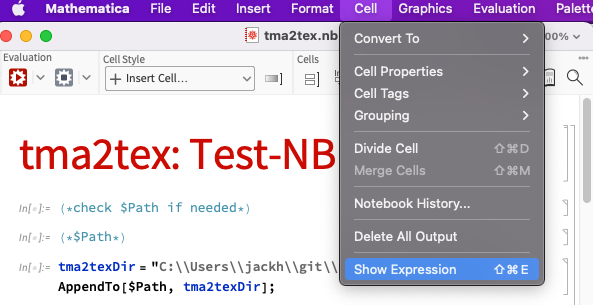
\includegraphics[scale=0.5]{images/introduction/MM-show-expression.png}
    \caption{In Mathematica Desktop, Cell menu and then "Show Expression" reveals ...}
    \label{fig:MM-show-expression}
\end{figure}

\begin{figure}[h]
    \centering
    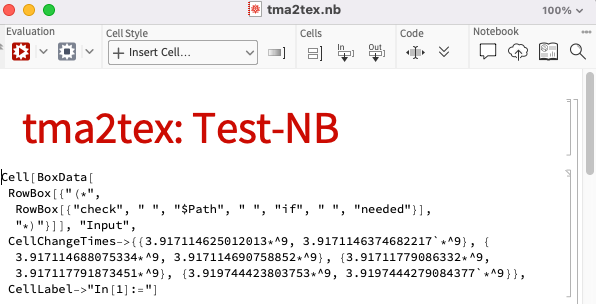
\includegraphics[scale=0.5]{images/introduction/MM-show-expression-1.png}
    \caption{... the lower level expression encoding the typesetting information for what is rendered by the front-end part of the system.}
    \label{fig:MM-show-expression-1}
\end{figure}

As in the FirstTour test notebook, the cells that make up the \lstinline+Notebook[]+ expression (collected in a list), mostly contain in \lstinline+BoxData[]+ and related structures (again, "low-level" representations \cite{noauthor_boxdatawolfram_nodate}), used for typesetting: 'When Wolfram Language expressions are displayed in notebooks, they are represented by two-dimensional typesetting structures of “boxes”' \cite{noauthor_find_nodate} - thus, the typesetting mechanism for Wolfram Language notebooks is the combination of these box structures, also expressions of course, with cell- and notebook-expressions. Any parsing on a notebook therefore takes place in relation to these basic structural elements.

\section{Motivation} \label{document-processing}

The motivation for this project is two-fold: First, \LaTeX is a standard widely used in technical and scientific communities, including journals of relevance to RISC, for example. Second, the native export functionality provided in Mathematica out of the box is not tailored to the Theorema background evaluation of formula representations despite their relevance to Theorema-publications. 

The status quo this project seeks to address is the labor-intensive, manual \LaTeX-preparation of formulae from Theorema notebooks for publication purposes.

\subsection{Need: The \LaTeX-Standard for Academic Publishing in Mathematical Disciplines}

The \LaTeX-typesetting software system is maintained by The Latex Project \cite{noauthor_latex_nodate}: In their words, "\LaTeX is the de facto standard for the communication and publication of scientific documents." \cite{noauthor_latex_nodate-1}

The current thesis is not so much about the format as it is about WL as an engineering tool for the Theorema context and transforming WL/Theorema-notebooks to this format, but the short form history and overview feature list of the system shall be included here: It is based on Donald E. Knuth’s TeX typesetting language, where LaTeX was first developed in 1985 by Leslie Lamport (the "La" in LaTeX), and currently by The LaTeX Project. \cite{noauthor_latex_nodate} 

The Latex Project lists the system's current set of features as follows \cite{noauthor_introduction_nodate}.

\begin{itemize}
    \item Typesetting journal articles, technical reports, books, and slide presentations.
    \item Control over large documents containing sectioning, cross-references, tables and figures.
    \item Typesetting of complex mathematical formulas.
    \item Advanced typesetting of mathematics with AMS (American Mathematical Society) LaTeX.
    \item Automatic generation of bibliographies and indexes.
    \item Multi-lingual typesetting.
    \item Inclusion of artwork, and process or spot colour.
    \item Using PostScript or Metafont fonts.
\end{itemize}

\subsection{Comparison to Existing Functionality in Mathematica} \label{intro:existing-functionality}

Mathematica provides native \LaTeX-export functionality, drawing on AMS-LaTeX, already listed in in the features of the system: AMS-LaTeX extensions are included in the standard LaTeX distribution, where the "amsmath part is an extension package for LaTeX that provides various features to facilitate writing math formulas and to improve the typographical quality of their output." \cite{noauthor_american_nodate} This can be shown by following the steps shown in Figures \ref{fig:MM-save-as} and \ref{fig:MM-to-latex} to save a notebook in in the \LaTeX-format in the "Save as ..." menu.

\begin{figure}[h]
    \centering
    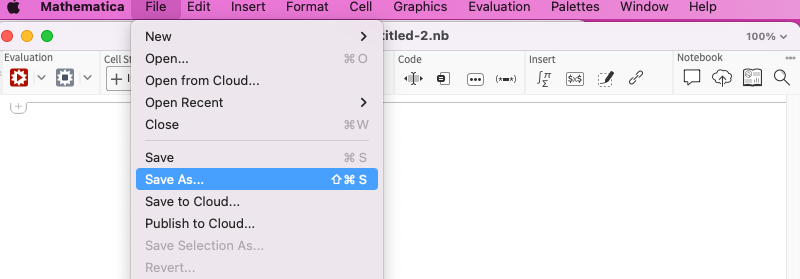
\includegraphics[scale=0.3]{images/introduction/MM-save-as.png}
    \caption{In Mathematica Desktop, file menu and then "Save as ..." leads to the option to save any notebook in \LaTeX format.}
    \label{fig:MM-save-as}
\end{figure}

\begin{figure}[h]
    \centering
    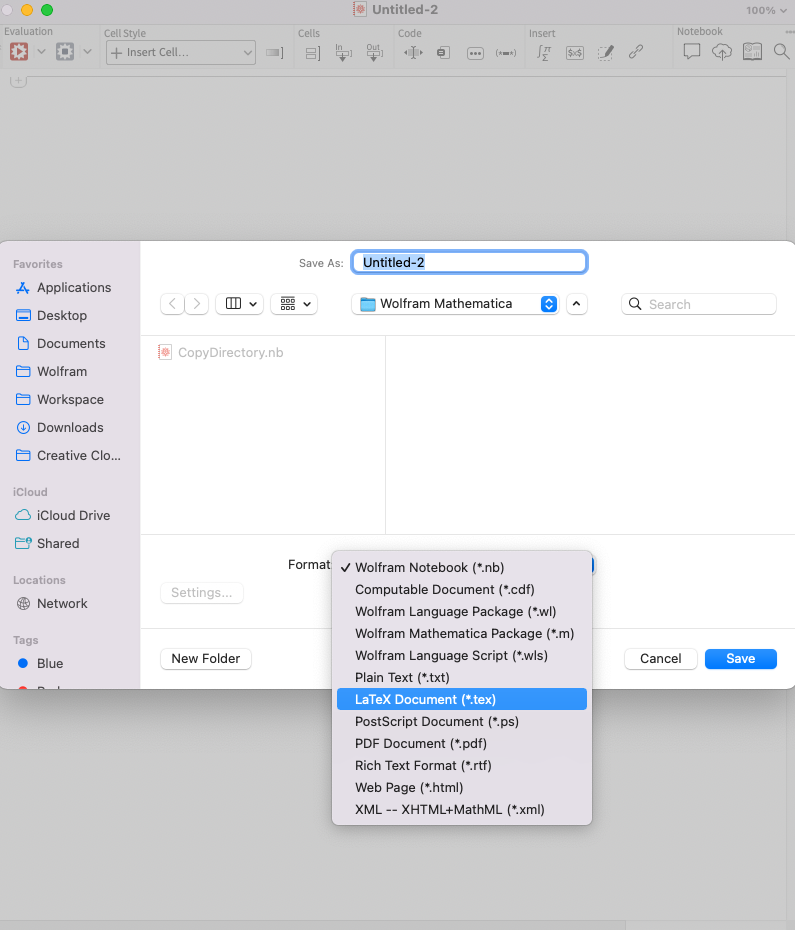
\includegraphics[scale=0.3]{images/introduction/MM-to-latex.png}
    \caption{There are also other export options next to default Mathematica notebook save option, and \LaTeX-Format, the option of interest at this point.}
    \label{fig:MM-to-latex}
\end{figure}

The .TeX-file produced consists of these lines, implementing related package imports and document setup commands.

\begin{verbatim}
%% AMS-LaTeX Created with the Wolfram Language : www.wolfram.com

\documentclass{article}
\usepackage{amsmath, amssymb, graphics, setspace}

\newcommand{\mathsym}[1]{{}}
\newcommand{\unicode}[1]{{}}

\newcounter{mathematicapage}
\begin{document}

\end{document}
\end{LaTeXCode}
\end{program}
\end{verbatim}

Crucially for this project, this native Mathematica solution does not work well for Theorema notebooks, as is easily seen when attempting to use this feature for this project's main test object, FirstTour.nb (provided in the project files), the PDF-rendering of the native \LaTeX-export (based on FirstTourNativeExport.tex, also provided in the project repository).

The WL (in-notebook) function TeXForm handles the cell-level transformation abd will be the basic Kernel-level functionality that is expanded upon to realize the fundamental transformation functionality in this project, discussed in Section \ref{concept:existing-functionality}.

\section{Development Environment}

\subsection{Tools Used}

In the present work, Mathematica and WolframKernel 14.1 \cite{noauthor_wolfram_nodate} are used throughout: Screenshots of Mathematica for desktop are used to show code evaluation where the frontend is relevant, and IntelliJ IDEA 2022.3.3 \cite{noauthor_intellij_nodate} is used in conjunction with the IntelliJ plugin Wolfram Language by Hal's Corner \cite{noauthor_wolfram_nodate-1} for syntax highlighting, as a guide for setting up a modern WL development environment and note on the present work's tooling: to reproduce this setup, simply install Mathematica (may require a license) and IntelliJ, then the plugin inside of the IntelliJ settings.


\subsection{Platform-(In)dependence}

Core concepts employed in this work to answer the challenge outlined in section \ref{document-processing}, for example pattern matching, related to the symbolic approach already discussed and explored in depth in Sections \ref{pattern-matching-concept} and \ref{pattern-matching-implementation}, are central to WL and the platform as a whole, making backwards and forwards compatibility within the Mathematica ecosystem highly likely. 

Since this work transforms Theorema documents and Theorema extends Wolfram Language, the tool developed here can be applied to vanilla Mathematica notebooks (Wolfram Language under the hood, that is, see section \ref{mm-vs-wl} on the relevant terminology) as well: The application requires execution on a compatible WL kernel setup. So, while the package is not, in principle, dependent on Theorema, and will simply transform available patterns in the input data - if these are not present, there is limited transformation - it is entirely dependent on the Wolfram Kernel included with Mathematica distributions.

On the level of the operating system, this implementation is platform-\textit{in}dependent and benefits from the Wolfram Language ecosystem setup (see criticisms in Section \ref{tool-chain-with-critique}) the way Theorema does, because (of) "Mathematica programs run without any modifications on essentially all available operating system platforms (Linux, OS X, and Windows), the powerful development group at Wolfram Research that keeps Mathematica being always an up-to-date platform growing into various directions, and the huge group of Mathematica users." \cite[p. 72]{windsteiger_theorema_2013}

\section{Mathematica/Wolfram Language Today}

\subsection{Mathematica vs Wolfram Language (vs Wolfram|Alpha)} \label{mm-vs-wl}

This disambiguation should be helpful for anyone new to the Wolfram ecosystem or "tech stack," as it is currently marketed: \cite{noauthor_wolfram_nodate}

\begin{itemize}
    \item Mathematica: the Desktop application, first introduced in 1988 and available for download in Version 14.1 currently. It is a proprietary technology available at a subscription cost. \cite{noauthor_wolfram_nodate-1}
    \item Wolfram Language: Frequently described as a "symbolic language," it is also the language that the Mathematica kernel is developed in and runs on. WL can be executed inside Mathematica. A Mathematica package typically has the file ending ".wl" (previously ".m") and can be called from inside Mathematica (a Mathematica notebook). It is also in principle closed source \cite{noauthor_wolfram_nodate} and available for licensing.
    \item Wolfram|Alpha: publicly available at no cost in the base version \cite{noauthor_wolframalpha_nodate} this product is sometimes conflated with Mathematica or Wolfram Language due to its public profile. "Wolfram|Alpha's long-term goal is to make all systematic knowledge immediately computable and accessible to everyone." \cite{wolfram_research_inc_about_2024}
\end{itemize}

\subsection{The Wolfram Tool Chain Today and Its Criticisms} \label{tool-chain-with-critique}

Mathematica, first appearing in 1988, is available in Version 14.1 at the time of writing and is being actively developed by Wolfram Research, with "new and improved" features (since Version 13.3) spanning topical categories like Mathematical Computation, Machine Learning and Neural Networks, High-Dimensional Visualization and Astronomy in addition to Core Language, Importing and Exporting and similar base categories. \cite{wolfram_research_export_nodate}] Mathematica, the Desktop application, continues to be Wolfram Research's core product, being marketed as the "world's definitive system for modern technical computing" \cite{noauthor_wolfram_nodate-1} and is distinguished from underlying technologies (Wolfram Language, Wolfram Cloud, Wolfram Knowledgebase, to name a few out of a longer list \cite{noauthor_wolfram_nodate-1}) and contrasts with the more unified platform approach of Wolfram|One \cite{noauthor_wolframone_nodate}, the publicly available Wolfram|Alpha \cite{noauthor_wolframalpha_nodate}, a set of mobile apps \cite{noauthor_wolfram_nodate} and further, more dedicated, products and services.

The size of the program and progress in development is typically measured in number of "in-built functions," that is, functions providing specific functionality, many levels of abstraction higher than the data structure and algorithm oriented functions provided by conventional languages and frameworks: see the following section \ref{computational-language} for the exploration of this idea. The current count of in-built functions, 6602 for the latest major release 14.0 \cite{wolfram_research_inc_summary_2024} and, for the newly released (minor) Version 14.1, up 89 to a new total of 6691 \cite{wolfram_research_inc_yet_2024}, with the trajectory since Version 1.0 in 1988 given in Figure \ref{fig:MM-number-of-built-in-functions}.

\begin{figure}[h]
    \centering
    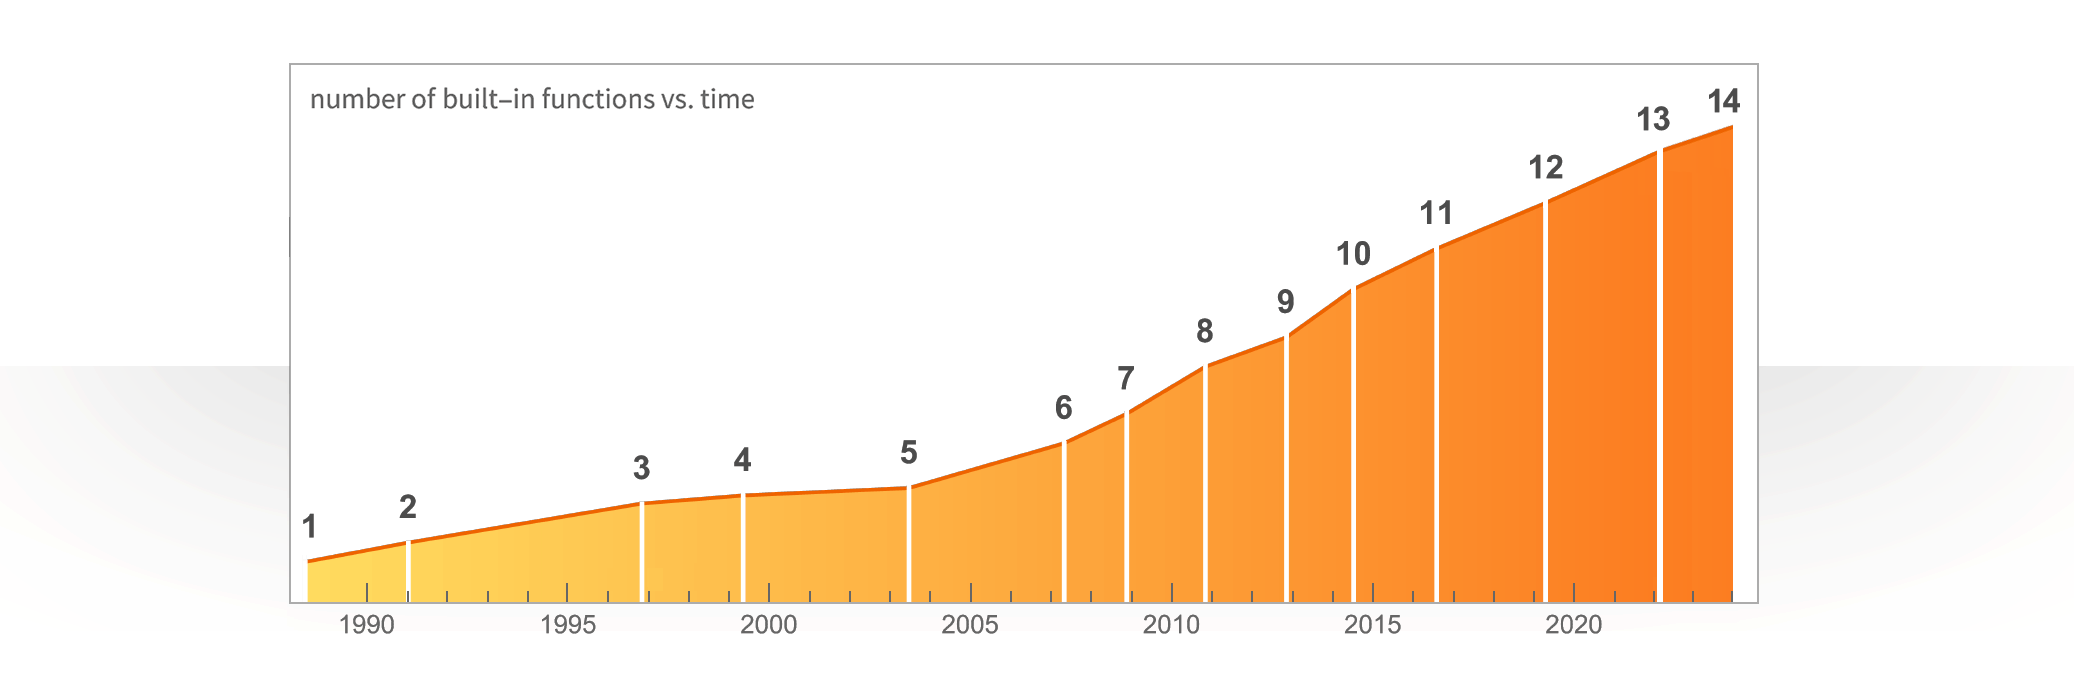
\includegraphics[scale=0.2]{images/introduction/stats-chart.png}
    \caption{In Mathematica Desktop, there are now over 6000 "built-in functions." \cite{noauthor_wolfram_nodate-1}}
    \label{fig:MM-number-of-built-in-functions}
\end{figure}

Criticism of the Wolfram products typically hinge on its closed-source, for-cost nature, though can also be extended to performance and trust in/vendor-lock-in with the company maintaining it, see for example \cite{noauthor_why_2022}. Specifically the former has been addressed as matters of philosophy when it comes to developing a programming language and associated ecosystem: "The simple answer is that large-scale, unified design requires centralized control and sustained effort that we feel is less achievable with free and open-source software" \cite{noauthor_wolfram_nodate} is the official customer facing answer in this proprietary context. A more extensive statement is given in \cite{noauthor_why_2019}, outlining 12 reasons for being closed-source, proprietary and at-cost, similar but slightly different aspects of this question.

Since this chapter started with Bruno Buchberger, I want to bring this particular question to his view, also mentioned in \cite{buchberger_mathematica_1996}: the professional development and marketing of Mathematica "is a feature that may have disadvantages for the research community because the code of the kernel of professional systems is normally not open for the user. On the other hand, it also provides some definite advantages as, for example, professional maintenance, high performance [!], professional software production tools, and - in the case of Mathematica - a fantastic front end." (p. 2) Buchberger was writing to Version 3.0 of Mathematica (in 1996) and is of course speaking of performance as it relates to efficient algorithms implemented in C that the kernel relies on, especially complex calculations "implementing the presently best mathematical methods in various fields" (p. 2), rather than performance as it pertains to the system and Mathematica kernel evaluations as a whole and how these might be compared against fully native C or other, lower level programming languages.

\subsection{How Wolfram Research Views Mathematica/Wolfram Language: The Computational Language Idea} \label{computational-language}

In addressing the question, "What Kind of a Thing Is the Wolfram Language?" \cite{noauthor_what_2019}, Stephen Wolfram, in some position to answer this, as the founder and current CEO of Wolfram Research and originator of the language, espouses the idea of a "computational" language, 'a way to apply the computational paradigm directly to almost anything: we have a language and a notation for doing computational X, for basically any field “X” (from archaeology to zoology, and beyond).' \cite{noauthor_what_2019} Such a multi-purpose tool is differentiated from conventional programming languages in the following way, relevant to the present work.

\begin{displayquote}
First and foremost, it’s that a computational language tries to intrinsically be able to talk about whatever one might think about in a computational way—while a programming language is set up to intrinsically talk only about things one can directly program a computer to do. So for example, a computational language can intrinsically talk about things in the real world—like the planet Mars or New York City or a chocolate chip cookie. A programming language can intrinsically talk only about abstract data structures in a computer. \cite{noauthor_what_2019}
\end{displayquote}

Mars \cite{noauthor_planetwolfram_nodate} and New York City \cite{noauthor_citywolfram_nodate} are examples of entities that can be addressed in WL using the so-called Wolfram Knowledgebase \cite{noauthor_wolfram_nodate}, which also powers Wolfram Alpha \cite{noauthor_curated_nodate}, another Wolfram Research product. The idea of the computational language turns on this easy access to data, as well as pre-built, high-level functions ("while the core of a standard programming language typically has perhaps a few tens of primitive functions built in, the Wolfram Language has more than 5600" at the time of writing \cite{noauthor_what_2019}, in 2019 - now 6602 in Mathematica and WL Version 14.1 \cite{noauthor_story_2024} in 2024, five years on) operating on the WL expression structure. 

This latter and the symbolic notion in an extended sense are seen as key in this presentation; to conclude it, and to give the intuition for the symbolic expressions and how they relate to the central pattern matching approach in Wolfram Language programming for processing expressions, not too different from Regular Expressions matching for strings (of text characters) in more conventional programming contexts: 

\begin{displayquote}
In most standard programming languages, x on its own without a value doesn’t mean anything; it has to stand for some structure in the memory of the computer. But in a computational language, one’s got to be able to have things that are purely symbolic, and that represent, for example, entities in the real world—that one can operate on just like any other kind of data.\cite{noauthor_what_2019}
\end{displayquote}

For the purposes of this work, in document transformation, where it has already been established that the document in question, a Mathematica notebook, is also such a symbolic expression, the idea simply means that any document following the (symbolic, that is expressions-)structure of a Theorema notebook can be processed using the Tma2TeX package: the symbolic in a symbolic expression is to mean something like a class of object, where their particular expression structure ("A foundational idea in the Wolfram Language is that all expressions—whatever they may represent—ultimately have a uniform tree-like structure," \cite{noauthor_expression_nodate}) including the individual expressions (their so-called expression "heads," \cite{noauthor_headwolfram_nodate}) match at the relevant level of abstraction. This level will be the defining mechanism that makes out the pattern matching approach, explored in the Theory chapter (\ref{cha:Theory}) in this work, Section \ref{symbolic-expressions}.

\subsection{The Connection to First Order Predicate Logic} \label{computational-language}

In propositional logic, 'the mathematical model of reasoning with statements composed logically from elementary statements (or propositions) [where] the only relevant characteristic of an elementary proposition (like “It rains.”) is that it can be true or false' \cite{jebelean_automated_nodate-1}, it is not possible to model predicates like "\( x \) is prime", nor can we reason about statements like "for all \( x \), there exists \( y \) such that \( y \) is a factor of \( x \)". \cite{michael_george_first_2024}

To handle these kinds of statements, predicates and quantifiers need to be introduced; this extended logic is referred to as predicate logic or first-order logic (FOPL):

\[
\phi \in \text{Formulae} ::= \dots \mid P(x_1, x_2, \dots) \mid \forall x, \phi \mid \exists x, \phi
\]

where \( x \) is drawn from a fixed set of variables. \cite{michael_george_first_2024}

Formally, an interpretation can be modeled as a set \( D \) and a function \( I : \text{Pred} \times D \times D \times D \times \dots \to \{T, F\} \) so that one can talk about the truth of a formula in a given interpretation. \cite{michael_george_first_2024}

WL, as a framework, aligns with FOPL, in the sense of the Computational Language concept already explored, leveraging the ability of users to express computational ideas at a high level, in a FOPL style, but providing the means to evaluate  expressions, integrating various data types and a sophisticated set of algorithms and front end, and other aspects of a "system for doing mathematics by computer" \cite{wolfram_research_inc_mathematica_2024}.
\chapter[Theoretical Background]{Theoretical Background: Theorema and Software Engineering, and the Project-Perspective on Programming Paradigms in Wolfram Language}
\label{cha:Theory}

This thesis already started off with rewriting-theory, so in this chapter I would like to focus the relevant insights from Theorema itself, as well as WL-systems-building and WL-paradigms, on practically relevant takeaways for the project part.

\section{Theorema} \label{tma}

Theorema is currently available in Version 2.0, under GPL \cite{noauthor_httpswww3riscjkuatresearchtheoremasoftware_nodate} and inlcuding the full source code on GitHub \cite{noauthor_github_nodate}. A tutorial is available as well. \cite{windsteiger_theorema_2017}

Relating the original goal of The Theorema Project with the current project, this foreword excerpt contextualizes Theorema in the world of theorem provers (as of 2006) by comparing the system to 16 others in the same class of system:

\begin{displayquote}
We can also see clearly from the examples in this collection that the notations
for input and output have to be made more human readable. Several systems do
generate LaTeX output for the discovered proofs, but perhaps additional thought
about formatting output might be valuable. The Theorema Project (system 12
in the present list) made readability of proofs a prime requirement, and their
report shows their success. However, the objective Prof. Bruno Buchberger set
originally for the project was to produce a tool for pedagogic use, not research.
\cite[p. 4]{g_mayrhofer_s_saminger__w_winsteiger_theorema_nodate}
\end{displayquote}

\subsection{Theorema vs Mathematica}

Just as we were interested in disambiguating Mathematica and Wolfram Language, to differentiate Theorema (Language) from the former two:

\begin{displayquote}
All Theorema ‘reasoners’ (provers, solvers, and simplifiers) are written in the programming language of Mathematica. Theorema does not use the Mathematica algorithm library or any implicit mathematical knowledge presupposed in Mathematica algorithms.
\cite[p. 110]{g_mayrhofer_s_saminger__w_winsteiger_theorema_nodate}
\end{displayquote}

In current speak, Theorema is implemented in Wolfram Language - but not using in-built algorithms or knowledge, such as the native experimental (in Version 14.0) functions \( ProofObject \) \cite{noauthor_proofobjectwolfram_nodate} and \( FindEquationalProof \) \cite{noauthor_findequationalproofwolfram_nodate}.

\subsection{\textit{Theorema 2.0} - Theorema Commander, Current Project Structure}

Theorema 2.0 most prominently introduces an interactive graphical user interface (GUI) to realize a full fledged mathematical assistant system, depicted in Figures \ref{fig:splash} (splash screen at application start), \ref{fig:start} (start screen under Windows) and \ref{fig:virtual-keyboard} (again the Theorema Commander, this time under Linux, taken from \cite{windsteiger_theorema_2013}), profiting from GUI-friendly dynamic expressions \cite[p. 76]{noauthor_introduction_nodate} and cascading stylesheets \cite{noauthor_stylesheetswolfram_nodate} both introduced with Mathematica Version 6 to realize a native implementation. The mode of interacting with the system fundamentally changes to be more newcomer friendly, because less relient on prior knowledge of the language:

\begin{figure}[h]
    \centering
    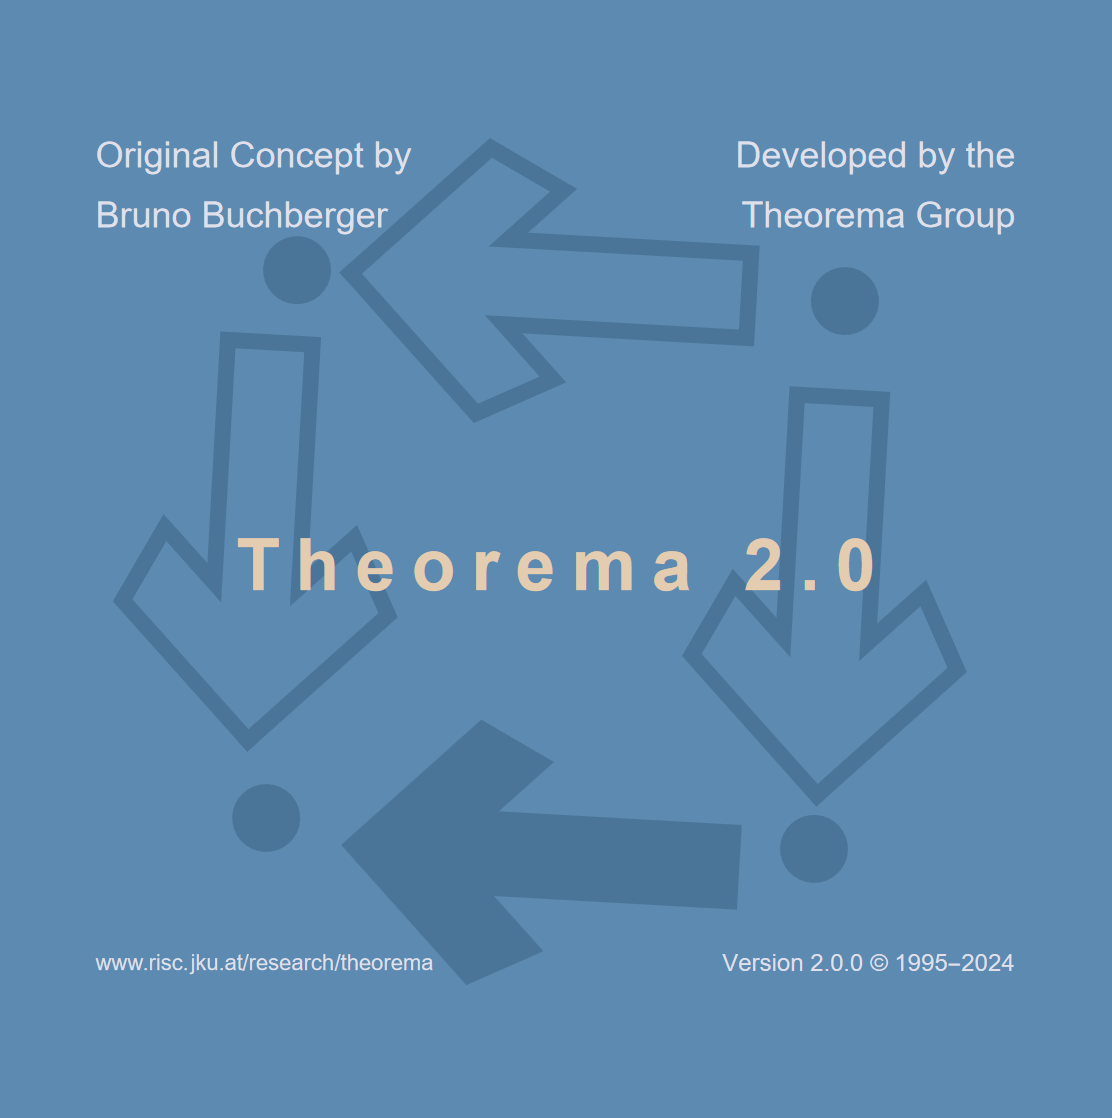
\includegraphics[scale=0.5]{images/theory/splash.png}
    \caption{The Theorema splash screen introducing the project and including a spinning RISC logo in the background.}
    \label{fig:splash}
\end{figure}

\begin{figure}[h]
    \centering
    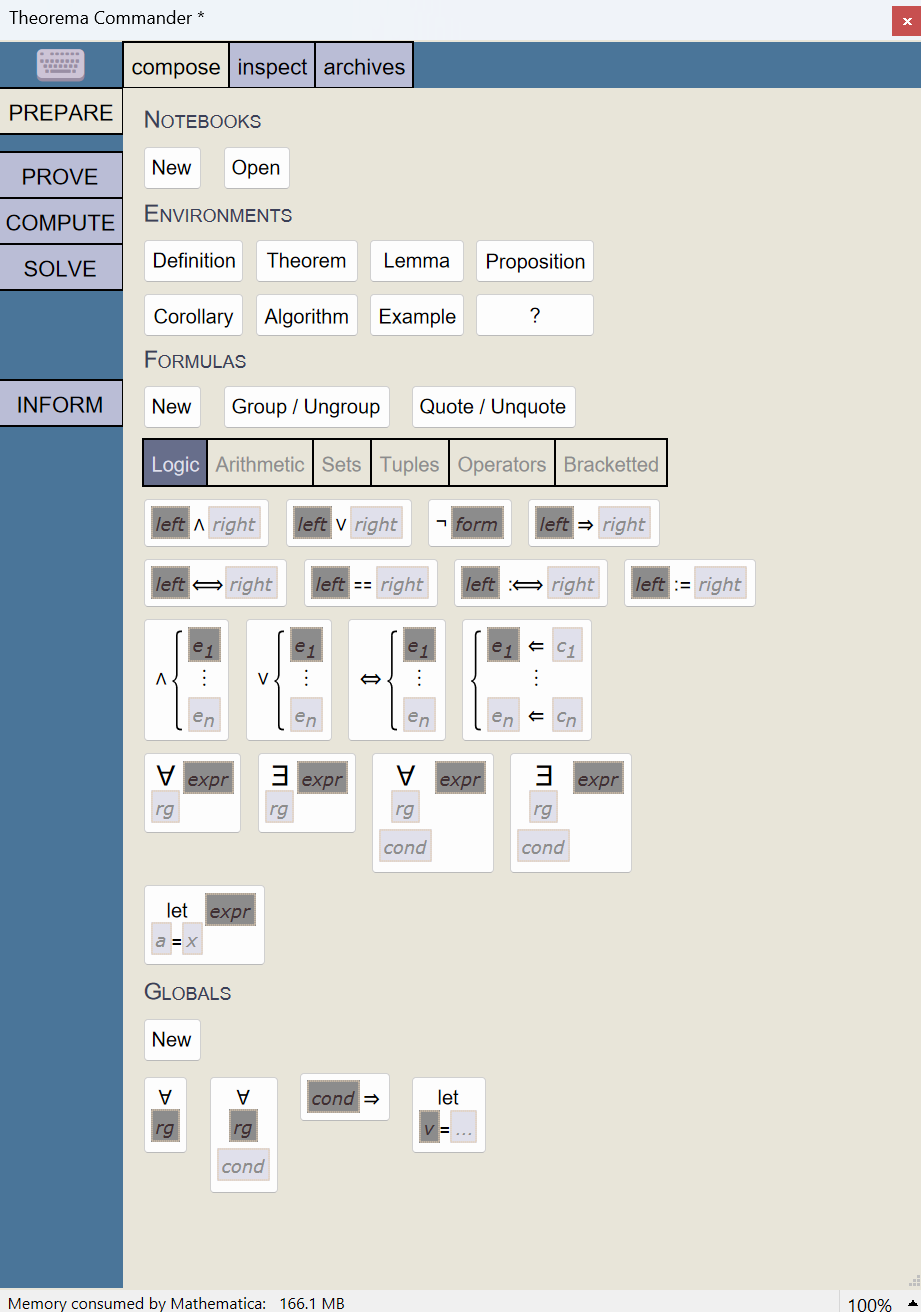
\includegraphics[scale=0.5]{images/theory/start.png}
    \caption{The start view in the Theorema Commander window: on Windows, the Commander opens in its own window, emulating an interface for a separate notebook.}
    \label{fig:start}
\end{figure}

\begin{figure}[h]
    \centering
    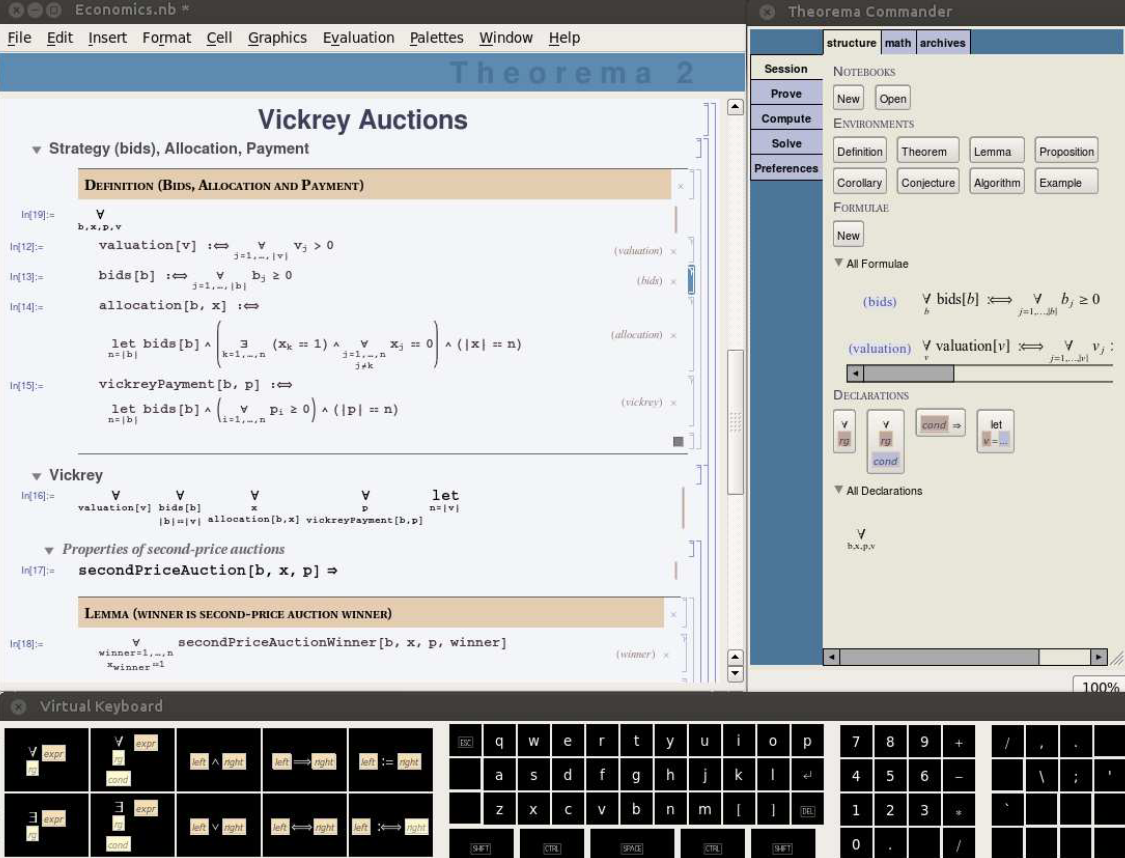
\includegraphics[scale=0.5]{images/theory/virtual-keyboard-linux.png}
    \caption{Taken from \cite{windsteiger_theorema_2013}, this side-by-side view of a notebook with the Commander also shows off the virtual keyboard, including "keys" for formula elements: comparing to the current version of the Commander in \ref{fig:start}, some changes have been made to the interface options, e.g. "Session" appears to be "Prepare"}
    \label{fig:virtual-keyboard}
\end{figure}

\begin{displayquote}
As an example, giving a definition meant evaluation of a \lstinline+Definition[...]+-command, stating a theorem meant evaluation of a \lstinline+Theorem[...]+-command, proving a theorem meant evaluation of a \lstinline+Prove[...]+-command, and performing a computation meant evaluation of a \lstinline+Compute[...]+-command. For the new Theorema 2.0 system, we envisage a more ‘point-and-click’-like interface as one is used to from modern software tools like a mail user agent or office software.
\cite[p. 73]{windsteiger_theorema_2013}
\end{displayquote}

The target user groups are mathematicians and students of mathematics \cite[p. 73]{windsteiger_theorema_2013} Since the Theorema provers are composed of smaller "special prover models" that can be recombined: "In the current status, the access to special prover modules is restricted to the system developers, but a mechanism for users to compose their own provers from available special prover modules is planned for future versions of the system." \cite[p. 111]{g_mayrhofer_s_saminger__w_winsteiger_theorema_nodate}

The current project structure is also made explicit in Figure \ref{tma-dir-tree}.

\subsection{The Logic of Theorema}

'The logic frame of Theorema is higher order
predicate logic, which is extended by the language construct “sequence variables,”' \cite[p. 110]{g_mayrhofer_s_saminger__w_winsteiger_theorema_nodate} already introduced in Section \ref{rewriting} and allowing for pattern matching capabilities. In this view, "the Theorema system is a (growing) collection of various general purpose and special theorem provers. The general purpose provers (like the first order predicate logic natural deduction prover) are valid only for special fragments of predicate logic (e.g. first order predicate logic)." \cite[p. 110]{g_mayrhofer_s_saminger__w_winsteiger_theorema_nodate} The more assumptions are made, the more specialized the prover module that is consulted.

The consequence of this theory for the current project of transforming Theorema documents is that the \LaTeX transformation target language needs to be able to represent Predicate Logic, and particularly, First Order Predicate Logic (FOPL).

\subsection{Theorema Environment and Surfacing the Theorema Language}

Theorema data is read from Mathematica notebooks \cite[p. 75]{windsteiger_theorema_2013}, but exists beyond the data directly visible in the front-end (this needs to be loaded at the appropriate time ahead of the \LaTeX-transformation, so that this authoritative form of the formula is the source of the transformation) - for display purposes, Theorema also defines specific stylesheets, changing the visual appearance from standard Mathematica notebooks, visible in Figure \ref{fig:virtual-keyboard}.

\begin{displayquote}
As soon as the [Theorema] formula is passed to the system through Mathematica’s standard Shift-Enter, the formula is stored in an internal datastructure that carries a unique key for each formula in addition to the formula itself and its label. This key consists of the absolute pathname of the notebook file in which it was given, and the unique cell-ID within that notebook, which is provided by the Mathematica front-end.
\cite[p. 75]{windsteiger_theorema_2013}
\end{displayquote}

We already saw a Theorema formula expression in the introductory chapter \ref{cha:Introduction}, Section \ref{tmaFormulaExpressionExample}: the structure starts like \lstinline+{Theorema`Common`FML$[{"ID:169304498", ...+ where we actually looking at a list of (denoted by curly braces) containing multiple \lstinline+Theorema`Common`FML$+ expressions, each in turn containing a list, and then some more data, but inside the list the first element is the unique cell-ID that the front-end provided. But, "the user never sees nor needs the concrete formula key explicitly." \cite[p. 75]{windsteiger_theorema_2013}

There is a hidden complication at this connection between front-end and internal datastructure: To capture the idea of a scope to make definitions in, Theorema allows for \textit{global declarations}, 'which may either contain one or several "orphaned" universal quantifiers (each containing a variable and an optional condition, but missing the formula, to which thery refer) or an "orphaned" implication (missing the right hand side), or an abbreviation indicated by a "let."' \cite{windsteiger_theorema_2013} names this biimplication:

\begin{center}
   \begin{displayquote}
    bids[\textit{b}] :\Longleftrightarrow \forall_{j=1,\cdots,|\textit{b}|} \textit{b}_j \geq 0
    \cite[p. 76]{windsteiger_theorema_2013}
    \end{displayquote} 
\end{center}

This actually translates to:

\begin{center}
    \begin{displayquote}
    \forall_\textit{b} bids[\textit{b}] :\Longleftrightarrow \forall_{j=1,\cdots,|\textit{b}|} \textit{b}_j \geq 0
    \cite[p. 76]{windsteiger_theorema_2013}
    \end{displayquote}
\end{center}

To make the idea specific to WL, an example from this project's main test notebook, FirstTour.nb, tracing such a declaration from its display in the front-end \ref{fig:global-decl}, to its notebook cell structure \ref{tmaGlobalDeclNotebookCell}, and finally, to its Theorema formula correlate \ref{tmaGlobalDeclFormula}, helps clarify this aspect of Theorema, relevant to the current goal of rendering an accurate output in \LaTeX: The question for the implementation will be how to obtain the Theorema-formula per relevant notebook cell and decide about a full length output (with global declarations) or a somehow trimmed version that is closer to the localized definition: further, it will likely be this hidden Theorema-representation we want to make visible by outputting the output document, rather than the purely-Wolfram-Language representation of the cell (structure) that holds the code for the display of the formula.

\begin{figure}[h]
    \centering
    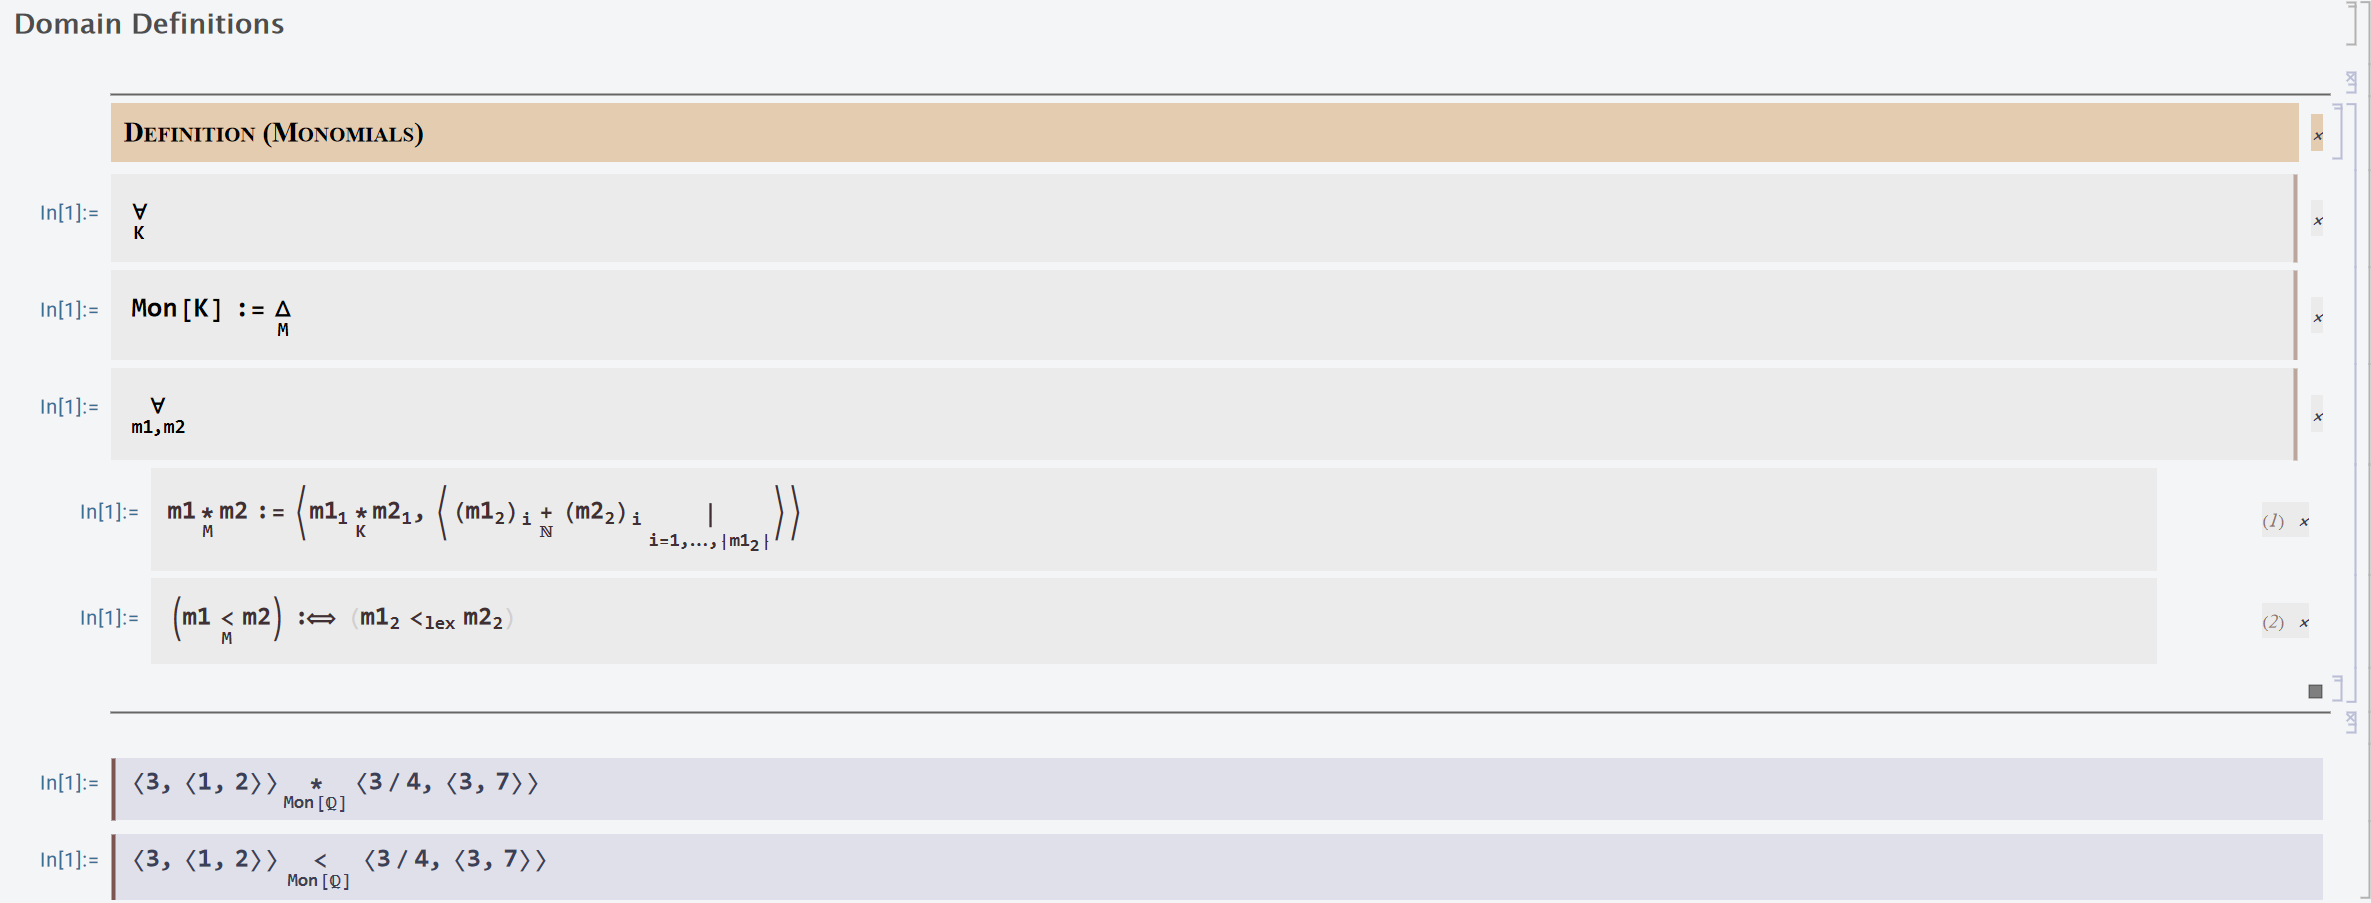
\includegraphics[scale=0.2]{images/theory/global-decl.png}
    \caption{A global declaration in Theorema with three different terms.}
    \label{fig:global-decl}
\end{figure}

\begin{program}
\caption{This is an excerpt from the notebook cell expression depicted in the front-end rendering in Figure \ref{fig:global-decl} and contains just one such global declaration, \lstinline+UnderscriptBox["\[ForAll]", "K"]]+ as the pertinent line from this cell structure.}
\label{tmaGlobalDeclNotebookCell}
\begin{LaTeXCode}
...
Cell[BoxData[
 UnderscriptBox["\[ForAll]", "K"]], "GlobalDeclaration",
 CellFrameLabels->{{None,
    Cell[
     BoxData[
      ButtonBox[
      "\[Times]", Evaluator -> Automatic, Appearance -> None, ButtonFunction :>
       Theorema`Language`Session`Private`removeGlobal[{
         "C:\\Users\\jackh\\OneDrive\\Documents\\RISC2023\\prototype-wolfram-\
lang\\FirstTour.nb", 2090454223}]]]]}, {None, None}},
 ShowCellTags->False,
 CellChangeTimes->{{3.62218621587292*^9, 3.622186218593838*^9}},
 EmphasizeSyntaxErrors->True,
 CellTags->"ID:2090454223",
 CellLabel->"In[1]:=",
 CellID->2090454223,ExpressionUUID->"809f4e1b-f26c-4265-a5d0-d66f43b5b903"]
...
\end{LaTeXCode}
\end{program}

\begin{program}
\caption{This is another Theorema formula and contains as part of it the global declaration term encoded in the notebook expression in \ref{tmaGlobalDeclNotebookCell}.}
\label{tmaGlobalDeclFormula}
\begin{LaTeXCode}
Theorema`Common`FML$[{"ID:2008910260", 
  "Source:C:\\Users\\jackh\\git\\repository\\tma2tex\\FirstTour.nb"}, 
 Theorema`Language`EqualDef$TM[
  Theorema`Language`DomainOperation$TM[Theorema`Knowledge`M$TM, 
    Theorema`Language`Times$TM][Theorema`Knowledge`m1$TM, 
   Theorema`Knowledge`m2$TM], 
  Theorema`Language`Tuple$TM[
   Theorema`Language`DomainOperation$TM[Theorema`Language`K$TM, 
     Theorema`Language`Times$TM][
    Theorema`Language`Subscript$TM[Theorema`Knowledge`m1$TM, 1], 
    Theorema`Language`Subscript$TM[Theorema`Knowledge`m2$TM, 1]], 
   Theorema`Language`TupleOf$TM[
    Theorema`Language`RNG$[
     Theorema`Language`STEPRNG$[
      Theorema`Language`VAR$[Theorema`Knowledge`VAR$i$TM], 1, 
      Theorema`Language`BracketingBar$TM[
       Theorema`Language`Subscript$TM[Theorema`Knowledge`m1$TM, 2]], 
      1]], True, 
    Theorema`Language`DomainOperation$TM[
      Theorema`Language`IntegerInterval$TM[1, \[Infinity], True, 
       False], Theorema`Language`Plus$TM][
     Theorema`Language`Subscript$TM[
      Theorema`Language`Subscript$TM[Theorema`Knowledge`m1$TM, 2], 
      Theorema`Language`VAR$[Theorema`Knowledge`VAR$i$TM]], 
     Theorema`Language`Subscript$TM[
      Theorema`Language`Subscript$TM[Theorema`Knowledge`m2$TM, 2], 
      Theorema`Language`VAR$[Theorema`Knowledge`VAR$i$TM]]]]]], "1"]
\end{LaTeXCode}
\end{program}

\section{Large Systems with Wolfram Language} \label{large-sytems}

Wolfram Research advocates for building large systems in WL and cites the WL system itself as "one of the more complex software systems ever constructed. It is built from several million lines of source code, written in C/C++, Java, and the Wolfram Language." \cite[The Software Engineering of the Wolfram System]{noauthor_internals_nodate} Wolfram Research cites the following general principles and more as they concern building large systems in any language \cite{noauthor_building_nodate}:

\begin{itemize}
    \item Divide the System into Components
    \item Write and Use Unit Tests
    \item Think of the Architecture, Not the Code
    \item Use Source Control
    \item Write Documentation
\end{itemize}

There are also WL-specific advantages in Software Engineering, explored in \cite[Take Advantage of the Wolfram Language]{noauthor_building_nodate}.

\subsection{Modularity with Packages} \label{modularity}

In WL, Package development \cite{noauthor_package_nodate}, namespace management \cite{noauthor_namespace_nodate}, and further scoping constructs \cite{noauthor_scoping_nodate} are interrelated and form the extensibility of the system: A typical Wolfram Language package is a .wl or .m file that contains a collection of functions and variables. These packages are structured in a way that separates the implementation from the interface, often using \lstinline+BeginPackage[]+ \cite{noauthor_endpackagewolfram_nodate} and \lstinline+EndPackage[]+ \cite{noauthor_endpackagewolfram_nodate} to define the public interface and \lstinline+Begin[]+ \cite{noauthor_beginwolfram_nodate} and \lstinline+End[]+ \cite{noauthor_endwolfram_nodate} for the implementation section.

Contexts are used to manage namespaces \cite{noauthor_namespace_nodate} , preventing name collisions between different packages or within different parts of the same package. By convention, package names serve as contexts, which helps in organizing the functions and variables and avoiding naming conflicts. Packages in the Wolfram Language use \lstinline+Get[]+ (\lstinline+<<+) \cite{noauthor_getwolfram_nodate} for loading, which executes the package code, effectively defining the functions and variables in the specified context. (\lstinline+Needs[]+ is the alternative, only loading loading the package if the specified context is not already in \lstinline+$Packages+, the relevant context variable in this case. \cite{noauthor_needswolfram_nodate})

\subsection{Theorema as an Extensible Mathematica Package} \label{extensible-package}

Theorema can be loaded like any WL-package but is really a collection of Wolfram Language packages, see \ref{tma-dir-tree} - the proposed format of the functionality implemented with this project is therefore also a WL-package, a file with file ending ".wl" (current) or ".m" (historically) and following the layout given by this Theorema template file ("Theorema
/PackageTemplate.m" \cite{noauthor_theorematheoremapackagetemplatem_nodate}) - including the copyright statement, which bakes the GNU (a recursive acronym, ""GNU's Not Unix:" The GNU Project was initiated by Richard Stallman in 1983 and is a free software, mass collaboration project \cite{noauthor_gnu_nodate-1}) licensing in right at the point of extensibility and states that anyone is free to redistribute and/or modify the software under the terms of the GPL (General Public License). \cite{noauthor_gnu_nodate} (However, the software is provided without any warranty.)

\begin{figure}[ht]
\centering
\vspace{10pt} % Adds 10 points of vertical space. Adjust the value as needed.
\begin{forest}
  for tree={
    font=\ttfamily,
    grow'=0,
    child anchor=west,
    parent anchor=south,
    anchor=west,
    calign=first,
    edge path={
      \noexpand\path [draw, \forestoption{edge}]
      (!u.south west) +(7.5pt,0) |- (.child anchor) \forestoption{edge label};
    },
    before typesetting nodes={
      if n=1
        {insert before={[,phantom]}}
        {}
    },
    fit=band,
    before computing xy={l=15pt},
  }
[Theorema
  [Computation]
  [Documentation
    [English]
  ]
  [FrontEnd]
  [Interface]
  [Kernel]
  [Knowledge]
  [Language]
  [Provers]
  [System]
]
\end{forest}
\caption{Directory Structure of the main directory in the Theorema project; directories are filled with .m-Mathematica/WL package files.}
\label{tma-dir-tree}
\end{figure}


\section{Paradigms: The Project-Perspective on the Multi-Paradigm Approach in Wolfram Language}

WL supports multiple programming paradigms, including the procedural one: "The Wolfram Language supports all standard procedural programming constructs, but often extends them through integration into its more general symbolic programming environment." \cite{noauthor_procedural_nodate} While not a pure OOP (Object Oriented Programming) language, WL can mimic OOP concepts through associative arrays (Associations) and symbolic structures, as outlined in Section \ref{oop}. 

\subsection{Functional vs Procedural Programming in Wolfram Language, and the High-Level Programming Paradigm} \label{high-level}

Functional programming in WL is introduced in the Wolfram Research documentation center as well \cite{noauthor_functional_nodate}, and exploring this in the context of high level programming is particularly fruitful, since the the combination of abstracted functionality with functional approaches can make for readable code. The present author would like to reference his exposé \ref{app:Expose} of the topic of contrasting these programming styles as they are applied to one particular example, Program \ref{treeProgram} and move on to the rule-based approach most relevant for the project at hand, after citing the seamless conversion of geometric objects to Unity (the game engine \cite{noauthor_real-time_nodate}) objects just one example of the high-level, abstracted idea of providing functionality in the WL ecosystem: 

\begin{center}
   \begin{displayquote}
    Drawing on its algorithmic power, Version 12 provides high–level functions that are uniquely easy to use to create and manipulate Unity objects. Easily create game objects with \lstinline+CreateUnityGameObject+ and directly include geospatial and socioeconomic data, and across thousands of domains.
    \cite{noauthor_highlevel_nodate}
    \end{displayquote} 
\end{center}

\begin{figure}[h]
    \centering
    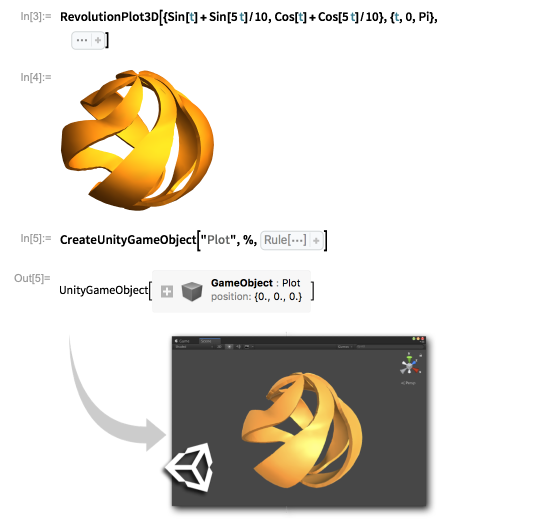
\includegraphics[scale=0.5]{images/theory/unity.png}
    \caption{Plots, graphics, and geometric objects are automatically converted to Unity's mesh format during the creation of a game object.\cite{noauthor_highlevel_nodate}}
    \label{fig:unity}
\end{figure}

Curated knowledge (data packages) available directly inside the WL system complement this paradigm-combination, as is made apparent in this example - see also Figure \ref{fig:unity}.

\begin{program}
\caption{These functions extract a tree data structure in the form of certain integer mathematical proof IDs and the related children IDs from a grid expression in WL and serve well to illustrate lists and replacements, functional and rule-based programming, as well as recursion, for efficient implementations. An expose with details is part of the appendix in the present work. \ref{app:Expose}}
\label{treeProgram}
\begin{LaTeXCode}
proofID[Grid[{___,{ID,id_},___},___]]:=id;
subproofs[
Grid[{___, {Proofs, OpenerView[{Arguments, Column[subproofs_, ___]}, ___]}, ___},
___]] := subproofs; subproofs[proof_] := {};
getLeanTree[proof_] := Tree[proofID[proof], getLeanTree /@ subproofs[proof], TreeElementLabelStyle  All  Directive[White, 16, FontFamily  "Times New Roman"], TreeElementStyle  All  Directive[EdgeForm[Black], RGBColor["#B6094A"]]]
\end{LaTeXCode}
\end{program}

\subsection{Symbolic Expressions Lead to Rule-Based Programming and Pattern Matching Approaches} \label{symbolic-expressions}

\subsection{Rule-Based Programming}

Another prominent mathematical research institute in Linz works with Mathematica \cite{noauthor_institute_nodate}, extending its rule-based programming capacity in the $\rho$Log package \cite{marin_rule-based_nodate} - much like Buchberger, Marin and Piroi identify Mathematica as a powerful system implementing the paradigm they are interested in, rule-based programming, the more general one as compared to (term) rewriting: While both concepts rely on rules, term rewriting is a specific type of rule-based operation focused on the transformation of expressions, whereas rule-based programming is a broader paradigm that can dictate various aspects of a program's behavior based on predefined logical rules.

This project's goals make the rule-based programming paradigm clearer. The author's outline the features lacking in Mathematica in terms of rule-based programming:

\begin{center}
    \begin{displayquote}
    \begin{enumerate}
        \item The possibility to program compositions of reductions, alternative choices, reflexive-transitive closures, etc.
        \item A built-in search mechanism to decide the existence of derivations $\text{Expr}_1$ $\rightarrow_{rr}$ $\text{Expr}_2$, where $\text{Expr}_1$, $\text{Expr}_2$ are given expression schemata (patterns), and $\rightarrow_{rr}$ is a specification of a sequence of rule reduction steps. Typically, the specification of $\rightarrow_{rr}$ is built with the operators mentioned before (composition, choices, etc.)
        \item The possibility to generate proofs which justify the existence or non-existence of such reduction derivations.
    \end{enumerate}
        \cite{marin_rule-based_nodate}
    \end{displayquote} 
\end{center}

To address these shortcomings, they simply implement a package to extend Mathematica according to their needs, achieving the following and demonstrating the flexibility of the system in this way.

\begin{center}
    \begin{displayquote}
    \begin{enumerate}
        \item Concise means to express the basic computational steps of an intended rule application as basic rules. These features are inherited from Mathematica, whose computational engine is based on a higher-order rewrite logic and with advanced support for symbolic and numeric computing.
        \item Programming constructs, such as conditional basic rules and rule combinators, which make it possible to structure large specifications of rules.
        \item Built-in search mechanism to answer queries of the form $\exists\{R_1,...,R_k\} \text{Expr}_1 \rightarrow_r \text{Expr}_2$ where $\text{Expr}_1$ is a ground expression, $r$ is the identifier of a rule, and $\text{Expr}_2$ is a Mathematica pattern whose variables are named $R_1, \ldots, R_k$ (see Section 2.2) [of \cite{marin_rule-based_nodate}].
        \item Support for generating proof objects, i.e., certificates that justify the correctness of the answer provided by $\rho$Log to a query.
        \item Visualization tools for proof objects, which enable the analysis of the deduction derivations of $\rho$Log in a natural language formulation and at various levels of detail.
    \end{enumerate}
        \cite{marin_rule-based_nodate}
    \end{displayquote} 
\end{center}

In both contexts, symbolic expressions are not just passive data; they are actively transformed or evaluated as part of the computational process. These expressions provide a versatile and powerful means to represent and manipulate knowledge, logic, and computations in a way that is abstracted from the specific details of the underlying data, allowing for more generalized and flexible rule application and system behavior.

\subsection{Rule-Based Programming vs Rewriting, via Pattern Matching}
\label{sec:rule_vs_rewriting}

Rule-based programming focuses on defining rules that guide the transformation of expressions within a program. It is declarative, meaning it specifies \textit{what} should be done rather than \textit{how} to do it. Rules are applied to expressions iteratively until no further rules can be applied or until a certain condition is met.

Pattern matching is a technique often used within rule-based programming but is more specifically focused on identifying parts of an expression that match a certain form. Pattern matching is integral to the process of identifying where and how rules should be applied in rule-based programming. Not all pattern matching is necessarily linked to rule-based programming.

Rewriting, while similar to rule-based programming, is a specific subset focused on the transformation of expressions through specific rules. It operates under the paradigm of applying these rules to achieve a specific form or outcome. Rewriting is a more specialized operation compared to the broader scope of rule-based programming.

\subsubsection*{Key Differences}
\begin{itemize}
    \item \textbf{Scope:} Rule-based programming can encompass various aspects of program behavior dictated by rules, whereas rewriting is a particular technique within this broader paradigm.
    \item \textbf{Focus:} Rule-based programming is concerned with defining transformations (the \textit{what}), while pattern matching focuses on identifying parts of an expression that need transformation (the \textit{identification}).
    \item \textbf{Application:} Pattern matching serves the rule-based programming paradigm by identifying where rules apply, while rule-based programming defines what transformations to apply.
\end{itemize}

\subsubsection*{Integration}
In the context of Wolfram Language and systems like Theorema, rule-based programming and pattern matching are core tools used to process and transform symbolic expressions. The interplay of these techniques allows for flexible and powerful manipulation of expressions, crucial for this project's task of converting mathematical expressions into \LaTeX.

\chapter{Concept: Package Design, Theorema Integration, TeXForm Consideration – In Any Case Pattern-Matching-Based Expression Processing}
\label{cha:Concept}

Having already taken a broad conceptual introductory approach and weighed the relevant theory, it should be efficient to derive the concept for a program package dealing with transformation of the notebook format to \LaTeX at this point: The aim is to apply the strengths of WL as a programming language as directly as possible.

\section{Conceptual Cornerstones for this Project}

\subsection{WL-Native Approach for Direct Integration with Theorema}

The design for the package is such that it is intended to be integrated with the Theorema project as a stand-alone package. Figure \ref{fig:hierary} illustrates the relationship of this package to Theorema (Language) and Wolfram Language, as a whole.

\begin{figure}[h]
    \centering
    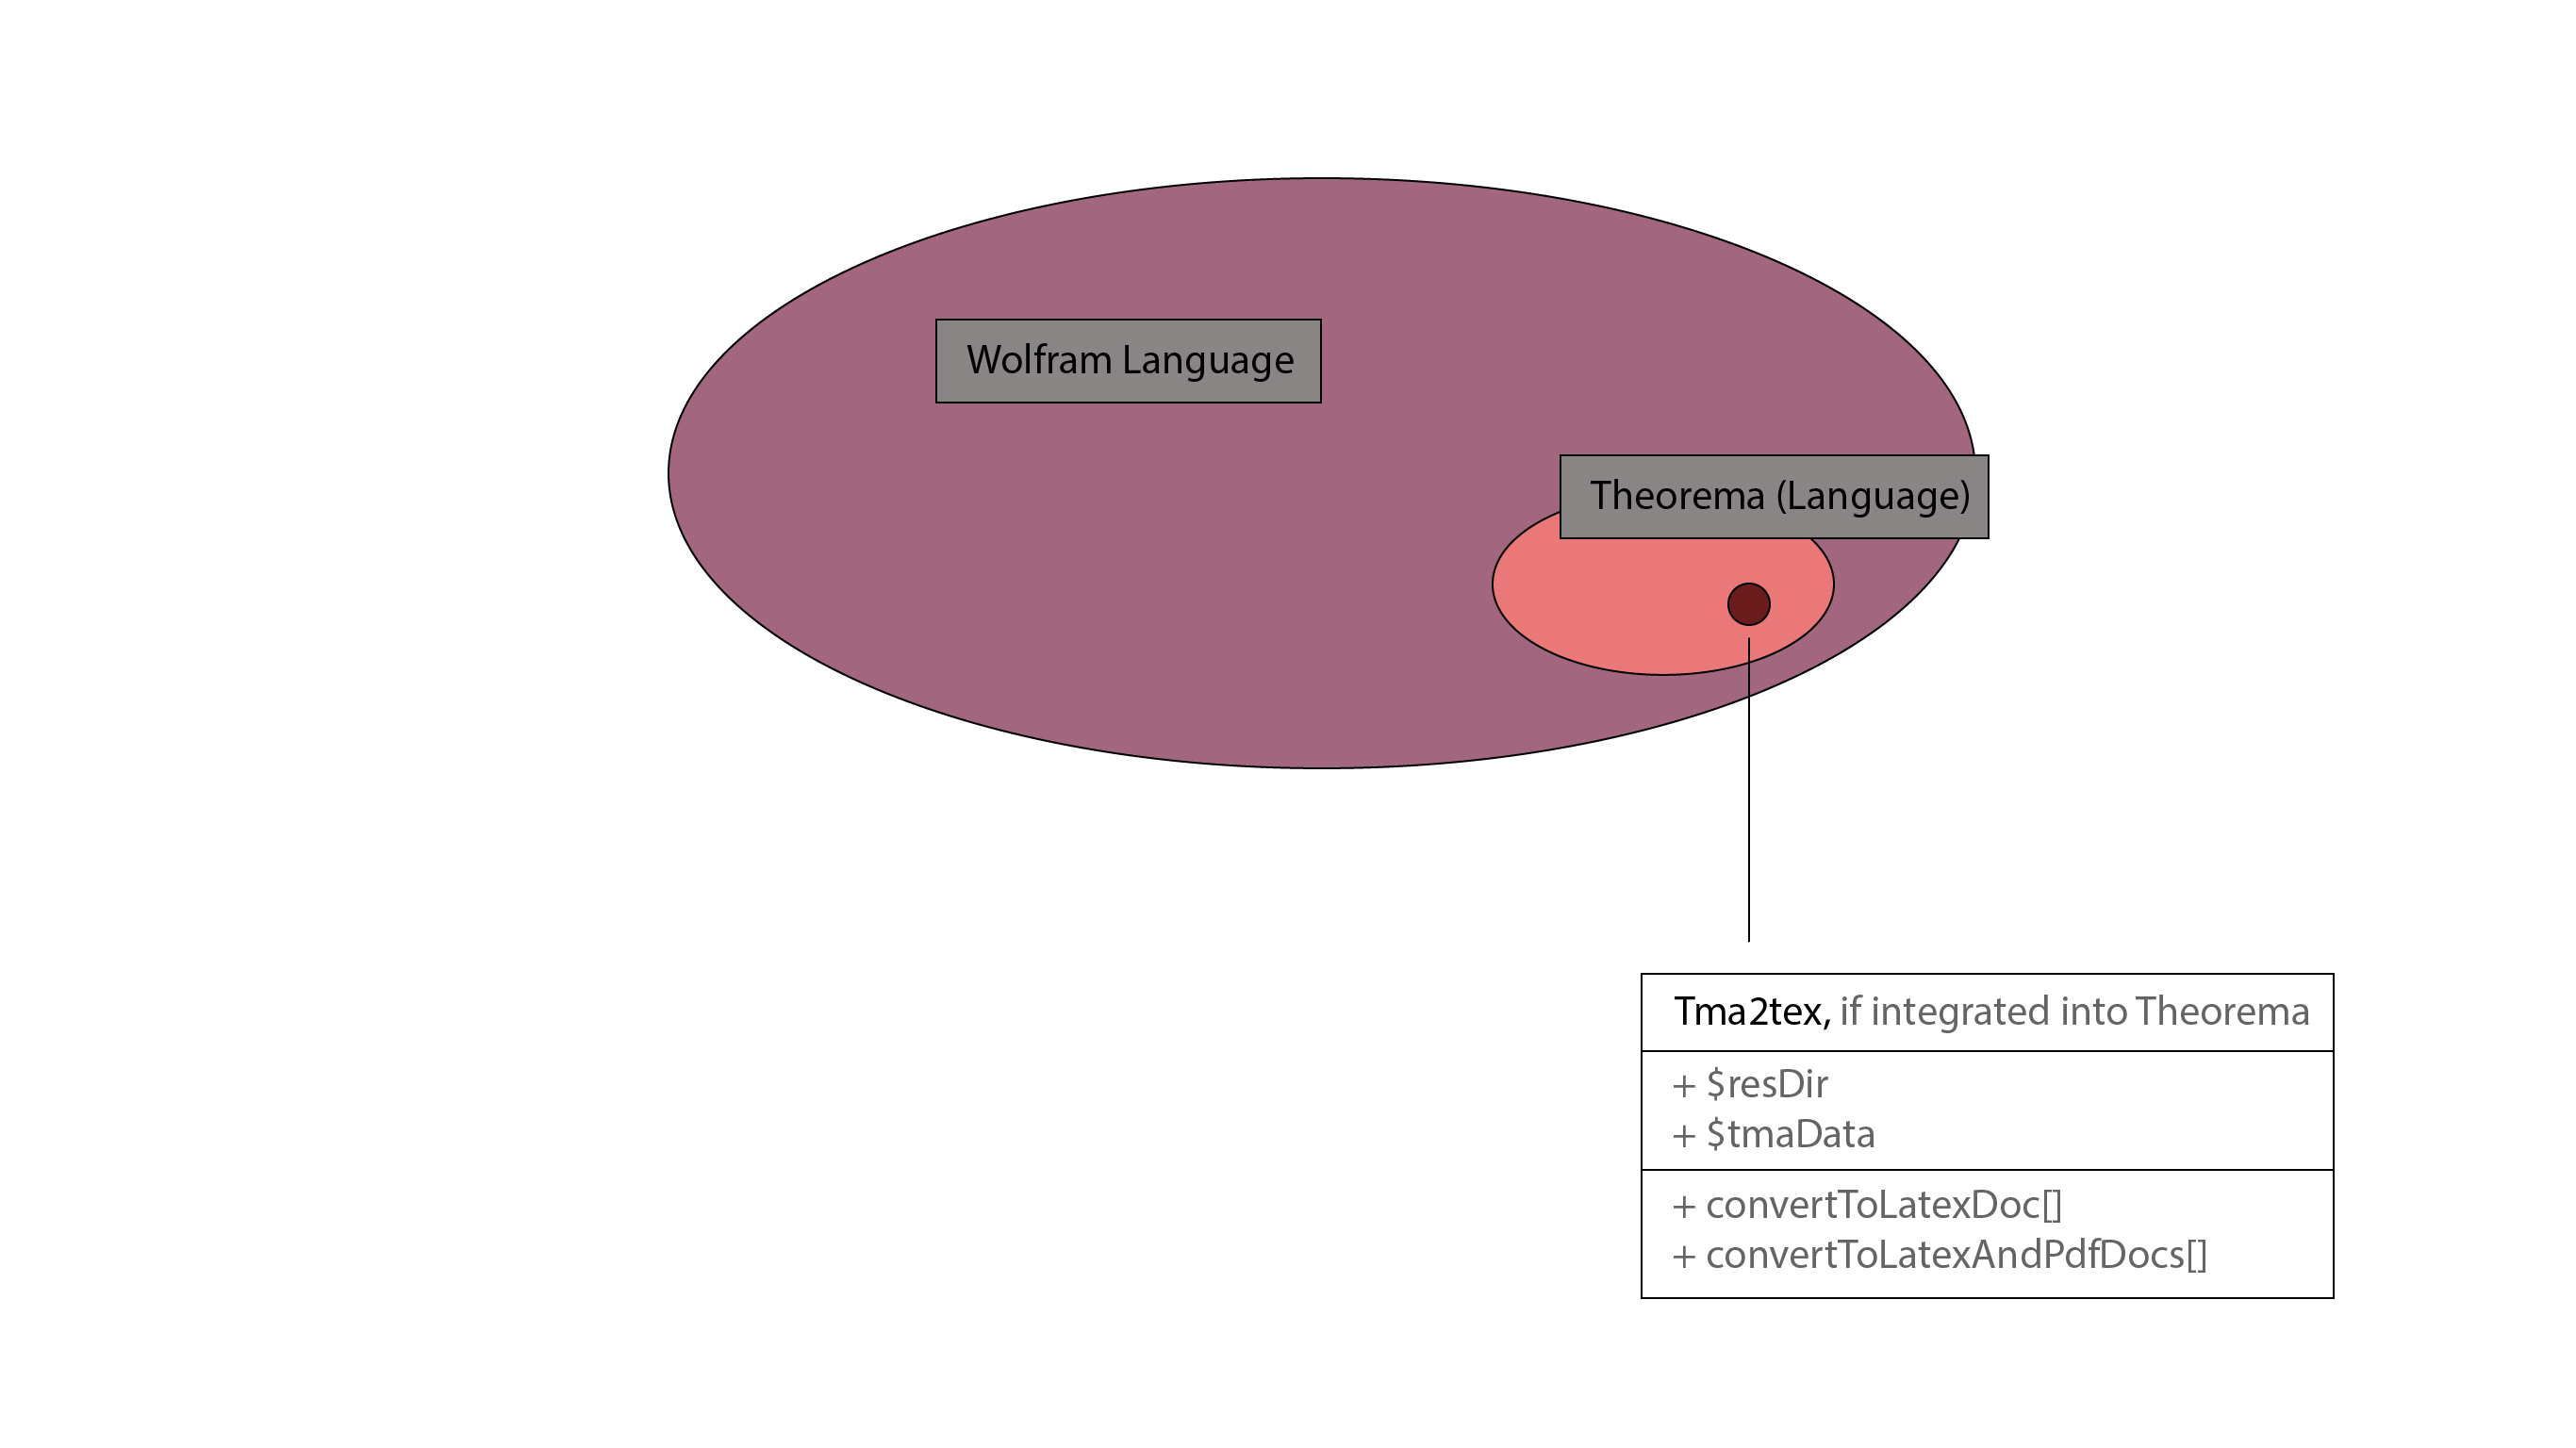
\includegraphics[scale=.35]{images/concept/Tma2Tex-Hierarchy.png}
    \caption{}
    \label{fig:hierary}
\end{figure}

The package itself is designed to follow the logic illustrated in Figure \ref{fig:package-logic}: files involved are colored green, code blue, transformation logic red - these are all the subject of this chapter.

\begin{figure}[h]
    \centering
    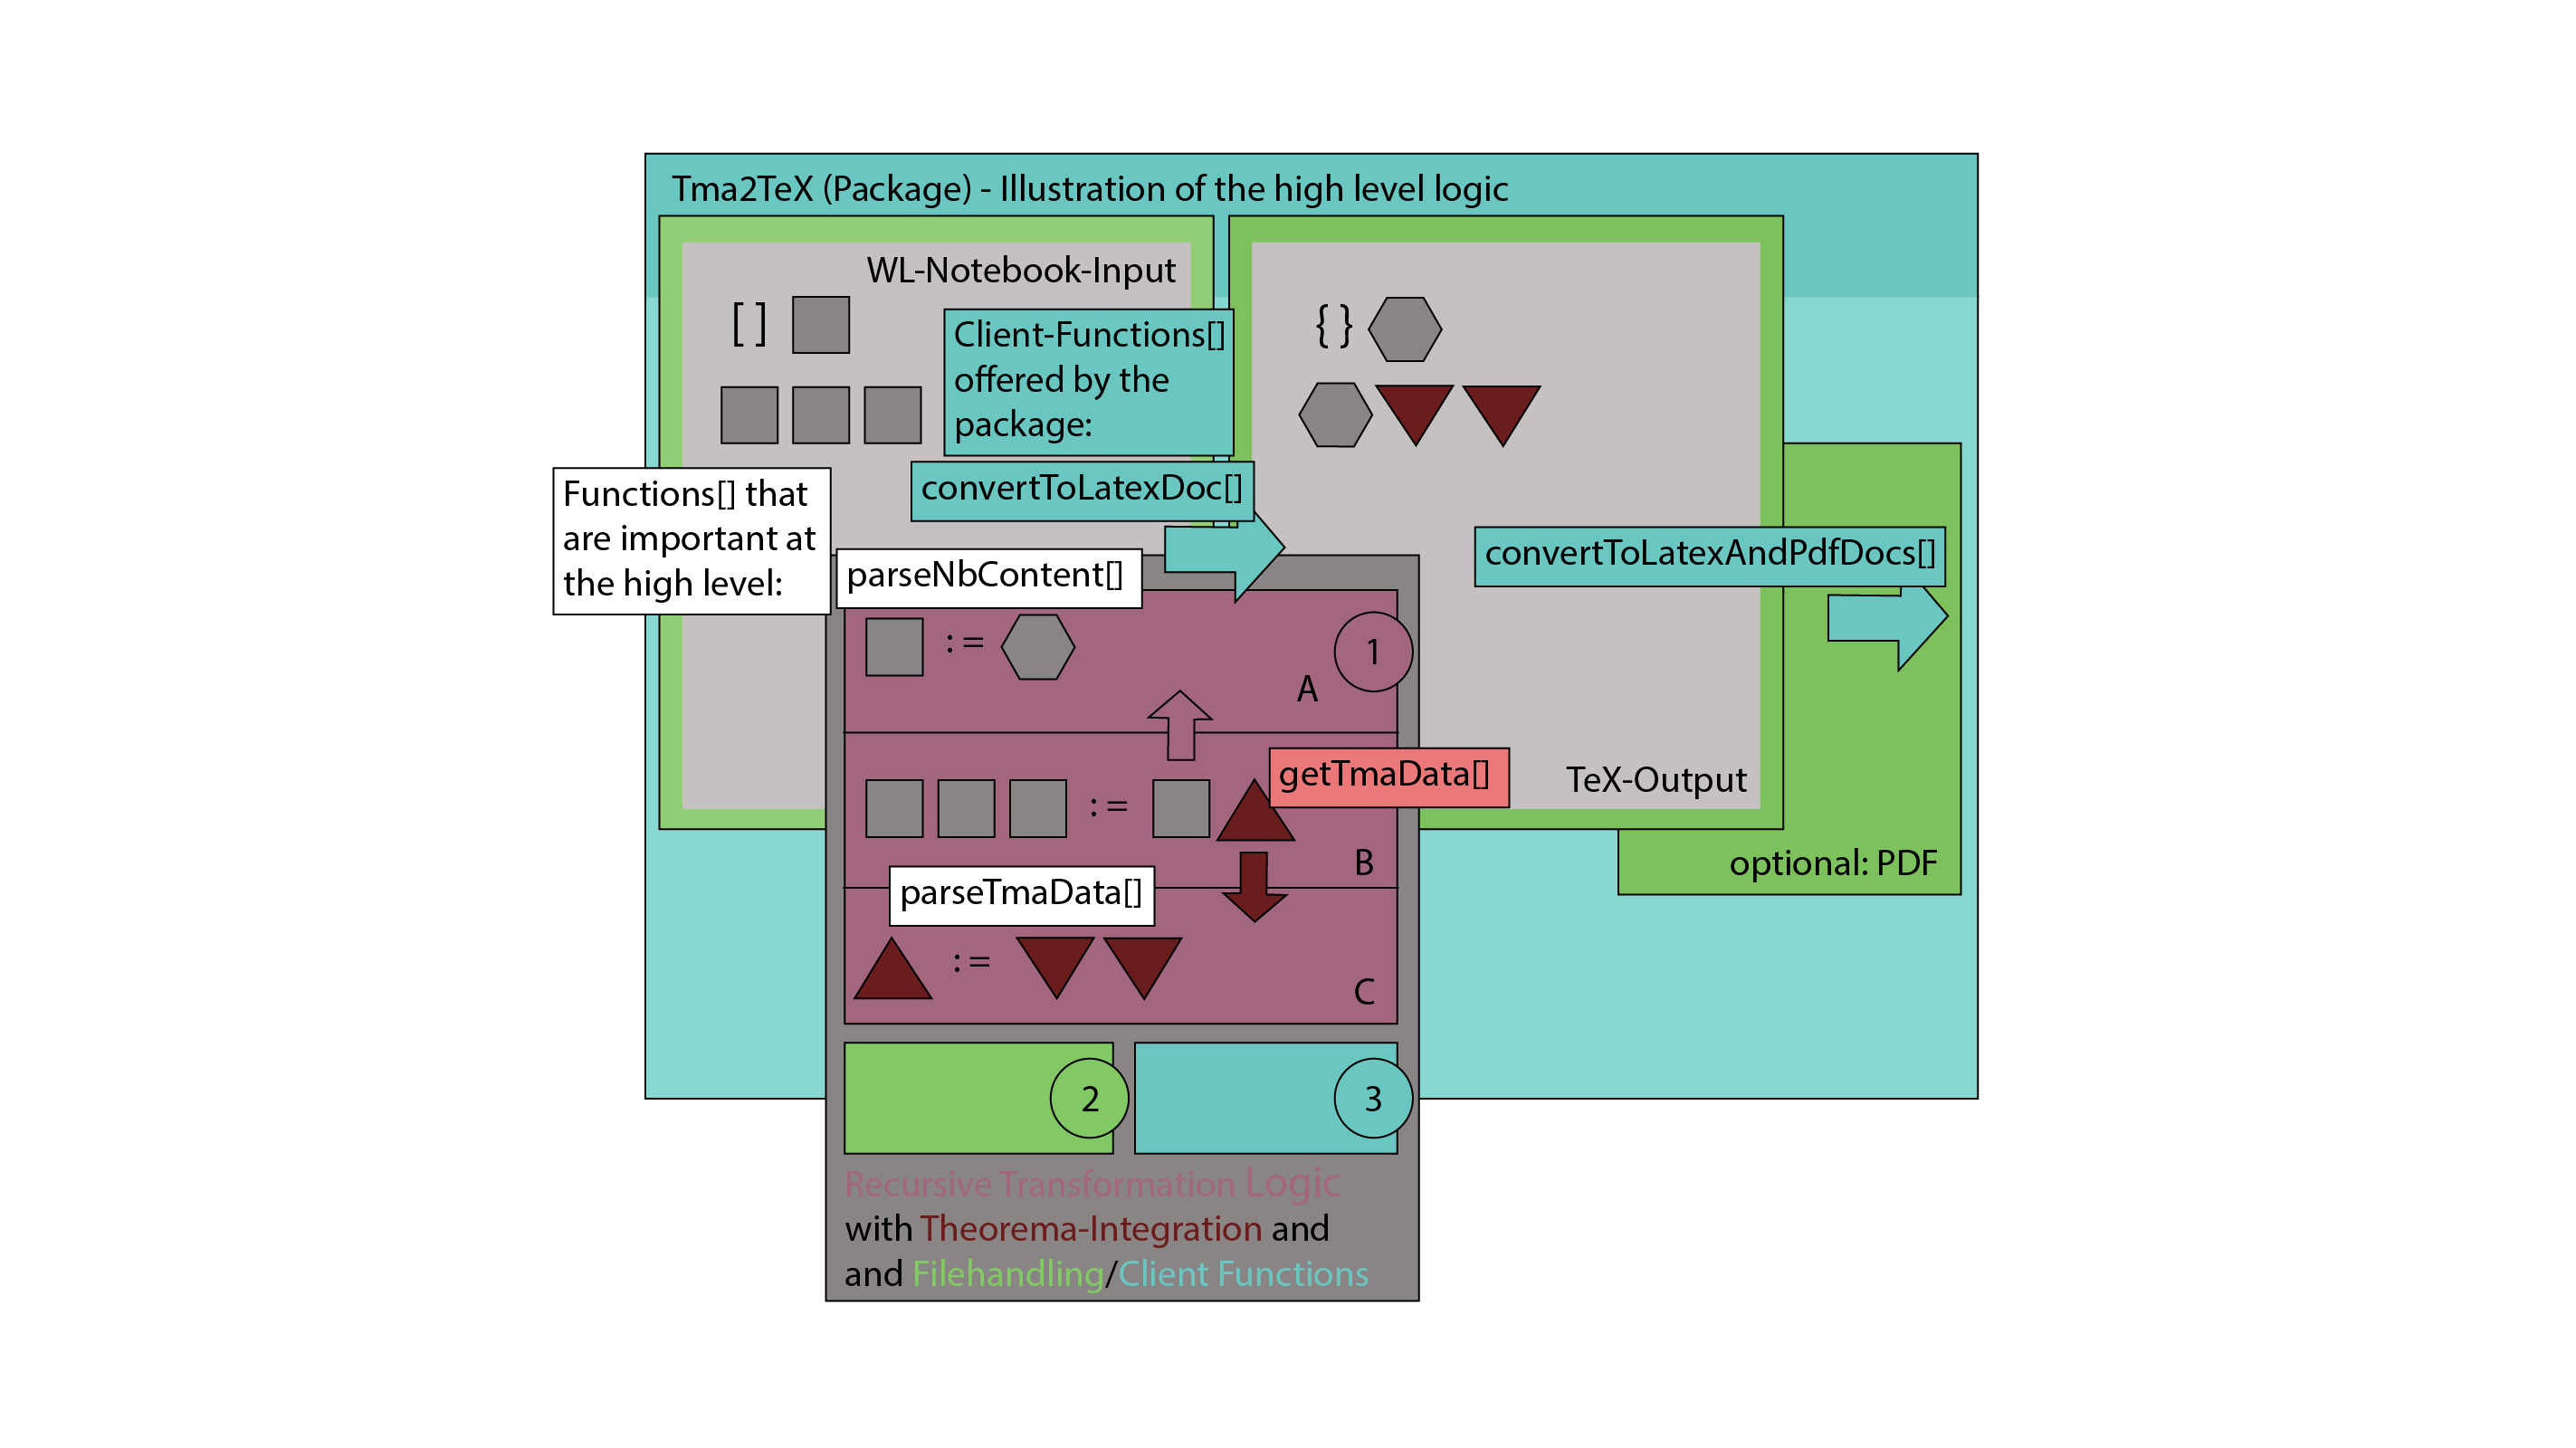
\includegraphics[scale=.35]{images/concept/Tma2Tex-Logic-01.png}
    \caption{}
    \label{fig:package-logic}
\end{figure}

This setup lends itself to an approach where the \LaTeX-template is used for customizations, at output: the template is filled by the \LaTeX generated by transforming the relevant Theorema Language formulas, particularly, but the Wolfram Language notebook as a whole, generally.

\subsection{Existing (Kernel) Functionality: Source Code Deep-Dive} \label{concept:existing-functionality}

The kernel sits at the core of the WL system (in keeping with the term in operating systems) and is available as a stand-alone program as well: "A standalone kernel session normally reads input from a device (typically a keyboard or a WSTP \cite{wolfram_research_inc_wstp_2024} connection), evaluates the expression and prints the result to a device (typically a screen or a WSTP connection)." \cite{wolfram_research_inc_wolframkernelwolfram_2024} Therefor the kernel needs to contain the main functionality expected for the WL system (independently of the notebook environment). From a software development standpoint, the kernel repository is the place to find the implementation for any essential function that a package outside of the kernel might rely on.

For this project, the main kernel function of relevance is TeXForm, which takes a WL expression and transforms it to its typesetting correlate in \LaTeX. Looking directly at the implementation reveals that the expedient way to handle this transformation is to exhaustively list and maintain the transformation rules in the form of a WL association. In order, the following categories (with one example each) make up most of the currently about 2000 lines of code inside the TeXForm package.

\begin{center}
    \begin{tabular}{||c c c||} 
         \hline
         Variable & Category of Symbol & Replacement Rule Example \\ [0.5ex] 
         \hline
         \hline
         \lstinline+$GreekLetters+ & Greek Letters & \lstinline+"\[Alpha]" -> "\\alpha "+ \\ 
         \hline
         \lstinline+$CaligraphicLetters+ & Caligraphy & \lstinline+"\[ScriptA]" -> "\\mathit{a}"+ \\
         \hline
         \lstinline+$GothicLetters+ & Gothic & \lstinline+"\[GothicA]" -> "\\mathfrak{a}"+ \\
         \hline
         \lstinline+$DoubleStruckLetters+ & Double-struck/Emphasis & \lstinline+"\[DoubleStruckA]" -> "\\mathbf{a}"+ \\
         \hline
         \lstinline+$AccentedLetters+ & Accented Letters & \lstinline+"\[AGrave]" -> "\\text{\\ a}"+ \\ [1ex] 
         \hline
         \lstinline+$MiscellaneousSymbols+ & Miscellaneous Symbols & \lstinline+"\[ConstantC]" -> "c"+ \\ 
         \hline
         \lstinline+$Shapes+ & Shapes & \lstinline+"\[FilledSquare]" -> "\\blacksquare"+ \\
         \hline
         \lstinline+$TextualForms+ & Special Characters & \lstinline+"\[DotlessI]" -> "\\text{\\i}"+ \\
         \hline
         \lstinline+$Operators+ & Operators & \lstinline+"\[Times]" -> "\\times"+ \\
         \hline
         \lstinline+$RelationSymbols+ & Symbols for Various Relations & \lstinline+"\[NotEqual]" -> "\\neq"+ \\ [1ex] 
         \hline
         \lstinline+$Arrows+ & Arrow-Symbols & \lstinline+"\[LeftArrow]" -> "\\leftarrow"+ \\ [1ex] 
         \hline
         \lstinline+$Spaces+ & Space-Characters & \lstinline+"\[ThickSpace]" -> "\\thickspace"+ \\ 
         \hline
         \lstinline+$Others+ & Other (Mathematical) Symbols & \lstinline+"\[Conjugate]" -> "*"+ \\
         \hline
         \lstinline+$LeftTeXDelimiterReplacements+ & Left Delimiters & \lstinline+"(" -> {"("}+ \\
         \hline
         \lstinline+$RightTeXDelimiterReplacements+ & Right Delimiters & \lstinline+")" -> {")"}+ \\
         \hline
         \lstinline+$TeXDelimiterReplacements+ & \LaTeX-Delimiters & \lstinline+"\\" -> {"\\backslash "}+ \\
         \hline
         \lstinline+$BasicEscapes+ & Escaped Characters & \lstinline+"#" -> "\\#"+ \\
         \hline
         \lstinline+$ASCIIUnchanged+ & ASCII characters & Function \\
         \hline
    \end{tabular}
\end{center}

This tabulation gives an idea of the type of transformations that would need to occur and implies for this project: while a mapping of a Theorema Language to WL expressions is possible in some cases (in fact a straightforward task in cases where the transformation is removing the suffix \lstinline+$TM+ and if needed, the full context with Theorema reference), any Theorema-to-\LaTeX transformation would be limited to symbols available in WL, negating the need and use of Theorema Language. Specific as-is output using notebook-level \LaTeX-transformation via file-export was already shown to be lacking in section \ref{intro:existing-functionality}.

Further, the pattern-matching-based \lstinline+parseNbContent+ allows for exactly the parts of the notebook of interest to the relevant user group, making the overall idea for the project a bespoke Theorema-TeXForm at notebook-level, in terms of existing WL-functionality, sitting neatly somewhere between a solution that solves expression-level TeX-transformation and notebook-level export.

As far as WL-TeXForm is concerned, all replacements are grouped together in an exhaustive list of replacements:

\begin{verbatim}
$TeXReplacements = Join[
  $ASCIIUnchanged, $BasicEscapes, $TeXDelimiterReplacements,
  $GreekLetters, (*$GreekWords,*) $AccentedLetters, $Spaces,
  $CaligraphicLetters, $GothicLetters, $DoubleStruckLetters,
  $MiscellaneousSymbols, $Shapes, $TextualForms,
  $Operators, $RelationSymbols, $Arrows, $Others
]
\end{verbatim}

These \lstinline+TeXReplacements+ inform the actual parsing in TeXForm. As has been argued already, TeXForm needs to be expanded in some way to permit Theorema-language parsing. Now a problem arises, however, because it is not as straightforward as a simple case-by-case switching between TeXForm and TheoremaTeXForm, say.

The (closed) source code for the Kernel would need to be opened to intertwine Theorema-specific functionality with TeXForm-functionality. This is illustrated by the fact that TexForm needs the complete expression to operate on successfully (maintaining correct nesting) and would not be useful called on an independent part (at any level in the expression hierarchy) individually: so \lstinline+TeXForm[And[Or[a,b], Or[c,d]]]+ would yield \lstinline+(a\\lor b)\\land (c\\lor d)+ natively, but called on the Theorema-language correlate at the outer level, that is \lstinline+ExpressionToTeX[And$TM[Or[a, b], Or[c, d]]]+, gives \lstinline+\\text{And$TM}(a\\lor b,c\\lor d)+: The text-rendering of unrecognized symbols is a sensible default. Calling a Theorema-version of TeXForm on only the And\$TM-expression, however, is problematic, because the TeXForm, as implemented in texformdump.wl and provided in the project repo, is fundamentally recursive to handle nested expressions. Without access to the way the operative recursive function (MakeTeX as it turns out) is called, a native-only TeXForm-solution would not work to handle Theorema language expressions in the proposed method.

The MakeTeX/makeTeX distinction is significant because it realizes the separation between the caller package and \verb+Texformdump`+, the package. makeTeX is the driver of the recursion-parsing, but calls MakeTeX in turn, which is only defined exactly once inside this base package, suggesting its usage to the user, the caller package:

\begin{verbatim}
(* Only built-in rule *)
MakeTeX[boxes_] := maketex[boxes]
\end{verbatim} 

Any overloading of MakeTeX overrides all corresponding maketex rules, so while it is important that maketex recursively calls MakeTeX, not maketex, maketex is doing the heavy lifting, and MakeTeX allows the user to override definitions at any expression level. MakeTeX-rules can also be defined inside the caller package in this way and it is by this mechanism that this project realizes the TeXForm-customization, building functionality into the natively used transformation rules and defaulting to this as needed, in the case of no special Theorema transformation rules targeting the corresponding LaTeX.

The process hinges on the functions MapTeX, the list-input version of MakeTeX - 

\begin{verbatim} 
MapTeX[stuff_List] := Map[MakeTeX, stuff]
MapTeX[stuff___] := MapTeX[{stuff}]
\end{verbatim} 

- as well as some auxiliary logic informing the central set of makeTeX functions making up the last quarter of the TeXForm implementation. The first makeTeX, for example, is:

\begin{verbatim}
maketex[RowBox[{l___, lb:DelimiterPattern, mid___, rb:DelimiterPattern, r___}]] :=
Module[{delimQ},
  DebugPrint["------------------------------------"];
  DebugPrint["maketex[RowBox[{l___, lb:DelimiterPattern, 
    mid___, rb:DelimiterPattern, r___}]]"];
  DebugPrint["l: ", l];
  DebugPrint["lb: ", lb];
  DebugPrint["mid: ", mid];
  DebugPrint["rb: ", rb];
  DebugPrint["r: ", r];
  delimQ = DelimiterBoxQ[mid];
  StringJoin[
    MapTeX[l],
    If[delimQ, InsertDelimiters["left", lb], MakeTeX[lb]],
    MapTeX[mid],
    If[delimQ, InsertDelimiters["right", rb], MakeTeX[rb]],
    MapTeX[r]
 ]
]
\end{verbatim}

\subsection{Package/MakeTeX-Specification} \label{concept:spec}

The following specification was developed in coordination with RISC and developed further as the project matured, especially as concerns extensibility (\verb+MakeTeX[]+):

\begin{itemize}

    \item \textbf{Package Dependencies:}
    \begin{itemize}
        \item \texttt{Theorema} (when not incorporated directly into Theorema, which is not part of this project and subject to user intention/Theorema development plan)
        \item If TeXForm-approximation were to be developed further: \texttt{Texformdump} 
    \end{itemize}
    
    \item \textbf{Global Variables:}
    \begin{itemize}
        \item \texttt{Tma2tex::\$resDir}
        \begin{itemize}
            \item \textbf{Usage:} Defines the directory for LaTeX-templates and any other resources.
            \item \textbf{Value in project repo:} \texttt{C:\textbackslash Users\textbackslash jackh\textbackslash git\textbackslash repository\textbackslash tma2tex\textbackslash res}
        \end{itemize}
        
        \item \texttt{Tma2tex::\$tmaData}
        \begin{itemize}
            \item \textbf{Usage:} Contains the Theorema-Datastructure that holds formula-expressions and is typically equivalent to \texttt{Theorema::Common::\$tmaEnv} on the Theorema-side but can be used to show the content according to Tma2Tex (as a separate package).
            \item \textbf{Value:} Subject to notebook loaded, e.g. FirstTour.nb (gives Theorema formula expressions, as a list, in Theorema language
        \end{itemize}
    \end{itemize}

    \item \textbf{Client-Functions:}
    \begin{itemize}
        \item \texttt{convertToLatexDoc}
        \begin{itemize}
            \item \textbf{Usage:} \texttt{convertToLatexDoc[notebookPath]} transforms a given WL notebook (by file path) to TeX output, creating a new TeX file from a specified resource template.
        \end{itemize}
        
        \item \texttt{convertToLatexAndPdfDocs}
        \begin{itemize}
            \item \textbf{Usage:} \texttt{convertToLatexAndPdfDocs[notebookPath]} transforms a given WL notebook (by file path) to PDF file as final output, with TeX file as intermediary step, from a specified resource template.
        \end{itemize}
        
        \item \texttt{convertToLatexFromString}
        \begin{itemize}
            \item \textbf{Usage:} \texttt{convertToLatexFromString[nbContentString\_, resourceDir\_Optional: Tma2tex::\$resDir]} is experimental and intended to be called from the Cloud, simply transforming Wolfram Language String Input to TeX Output (returned directly, not via file). Also uses a template, the resource for which can be passed as the second argument.
        \end{itemize}
    \end{itemize}

    \item \textbf{Lower Level Functions}, provided to the user in the case of TeXForm-approximation - this alternative approach, hinging on a MakeBoxes, a function to create a \"boxes\"-representation as an intermediary step, is discussed in section \ref{concept:pipeline}. This approach would benefit from the following specification.
    \begin{itemize}
        \item \texttt{boxesToTeX[boxes\_]}, to transform a cell-level boxed expression
        \item \texttt{expressionToTeX[expr\_]}, to transform cell-level expressions (uses MakeBoxes \cite{wolfram_research_inc_makeboxeswolfram_nodate} in the background, in Texformdump-package, to then pass to Texformdump`boxesToTeX in the end) 
        % Potential TODO: elaborate on Standardform MakeBoxes vs Theoremaform Makeboxes and TEST if Theorema-form MakeBoxes -> boxesToTeX works
        \item \texttt{makeTex[boxes\_]}, for adding custom box-level transformation rules
        %\item [TODO:] \texttt{MakeTeX[\{..->..\}]} for adding rules, as an association, where anything suffixed by \texttt{\$TM} is a custom Theorema rule generated to the resource template from the WL side, in code.
        %\item [TODO:] \texttt{MakeTeX[..\$TM\_String or list of \$TM-suffixed strings]} being a list of customizations expected as rules inside the template: so the actual \LaTeX command is expected to be specified on that end.
        \item \texttt{makeTex[string\_?isTmaCommand]}, for adding custom Theorema-command-level typsetting instructions, in the form of a \texttt{\\stringTM}-named \LaTeX command in tmaTemplate, e.g. \verb|\newcommand{\ForallTM}[2]{\forall_{#1} #2}| where \texttt{string} takes on the value \texttt{Forall}.
    \end{itemize}

\end{itemize}

These would essentially form the head of the package - see the overall notes on package design to conclude this chapter, \ref{paclet-design} - and all become available to the user, where it is anticipated that mostly the higher level functions, convertToLatexDoc and convertToLatexAndPdfDocs, will be of interest, and lowever level MakeTex only secondarily for specific cell transformations as needed, or for customizations of the transformation, and especially for users well-aquaited with the package.

\subsection{For This Project: No Layout-Information in the \LaTeX} \label{concept:our-approach}

Having considered the native TeXForm implementation and its reliance on native MakeBoxes, the approach taken here can now be appreciated in its difference: the core idea is to not include layout information of the type that is provided by MakeBoxes in generating the \LaTeX, but to work directly with the Theorema-Formula and give the user complete control over layout via \LaTeX and specifically the macros defined in-template.

A comparison will best illustrate the difference, first considering a Theorema formula and the desired output, and then a native WL expression, the relevant MakeBoxes-intermediate step, and the final TeXForm generated \LaTeX-output.

A Theorema formula:

\begin{verbatim}
 Theorema`Language`Iff$TM[
  Theorema`Language`And$TM[
   Theorema`Language`Forall$TM[
    Theorema`Language`RNG$[
     Theorema`Language`SIMPRNG$[
      Theorema`Language`VAR$[Theorema`Knowledge`VAR$x$TM]]], True, 
    Theorema`Language`Or$TM[
     Theorema`Knowledge`P$TM[
      Theorema`Language`VAR$[Theorema`Knowledge`VAR$x$TM]], 
     Theorema`Knowledge`Q$TM[
      Theorema`Language`VAR$[Theorema`Knowledge`VAR$x$TM]]]], 
   Theorema`Language`Forall$TM[
    Theorema`Language`RNG$[
     Theorema`Language`SIMPRNG$[
      Theorema`Language`VAR$[Theorema`Knowledge`VAR$y$TM]]], True, 
    Theorema`Language`Implies$TM[
     Theorema`Knowledge`P$TM[
      Theorema`Language`VAR$[Theorema`Knowledge`VAR$y$TM]], 
     Theorema`Knowledge`Q$TM[
      Theorema`Language`VAR$[Theorema`Knowledge`VAR$y$TM]]]]], 
  Theorema`Language`Forall$TM[
   Theorema`Language`RNG$[
    Theorema`Language`SIMPRNG$[
     Theorema`Language`VAR$[Theorema`Knowledge`VAR$x$TM]]], True, 
   Theorema`Knowledge`Q$TM[
    Theorema`Language`VAR$[Theorema`Knowledge`VAR$x$TM]]]]
\end{verbatim}

The Theorema-MakeBoxes result:

\begin{verbatim}
 FormBox[
       RowBox[{
         RowBox[{"(", 
           RowBox[{
             RowBox[{
               UnderscriptBox["\[ForAll]", 
                RowBox[{
                  StyleBox["x", "ExpressionVariable"]}]], 
               RowBox[{
                 RowBox[{"P", "[", 
                   StyleBox["x", "ExpressionVariable"], "]"}], "\[Or]", 
                 RowBox[{"Q", "[", 
                   StyleBox["x", "ExpressionVariable"], "]"}]}]}], "\[And]", 
             RowBox[{
               UnderscriptBox["\[ForAll]", 
                RowBox[{
                  StyleBox["y", "ExpressionVariable"]}]], 
               RowBox[{
                 RowBox[{"P", "[", 
                   StyleBox["y", "ExpressionVariable"], "]"}], "\[Implies]", 
                 RowBox[{"Q", "[", 
                   StyleBox["y", "ExpressionVariable"], "]"}]}]}]}], ")"}], 
         "\[DoubleLeftRightArrow]", 
         RowBox[{
           UnderscriptBox["\[ForAll]", 
            RowBox[{
              StyleBox["x", "ExpressionVariable"]}]], 
           RowBox[{"Q", "[", 
             StyleBox["x", "ExpressionVariable"], "]"}]}]}], TheoremaForm]
\end{verbatim}

Applying TeXForm (in a modified version available in the file \lstinline+tma2texV0.wl+) would give:

\begin{verbatim}
    \left(\underset{x}{\forall }P[x]\lor Q[x]\land 
    \underset{y}{\forall }P[y]\Rightarrow Q[y]\right)\Leftrightarrow 
    \underset{x}{\forall }Q[x]
\end{verbatim}

However, the goal (as defined by the user) actually is:

\begin{verbatim}
    \IffTM{ \AndTM{ \ForallTM{ \RNGTM{ \SIMPRNGTM{ \VARTM{x}}}}{ \OrTM{ P[ 
    \VARTM{x}]}{ Q[ \VARTM{x}]}}}{ \ForallTM{ \RNGTM{ \SIMPRNGTM{ \VARTM{y}}}}{ 
    \ImpliesTM{ P[ \VARTM{y}]}{ Q[\VARTM{y}]}}}}{ \ForallTM{ 
    \RNGTM{ \SIMPRNGTM{ \VARTM{x}}}}{ Q[ \VARTM{x}]}}
\end{verbatim}

That is, the formula structure should be translated directly to customizable Theorema-specific commands, and not actually assume any layout information whatsoever, the way TeXForm approaches the problem.

\subsection{MakeBoxes: An Alternative Typesetting-Pipeline} \label{concept:pipeline}

Both the Theorema and the TeXForm packages provide MakeBoxes-functionality \cite{noauthor_makeboxeswolfram_nodate}, taking care of the Mathematica typesetting: underscripts, delimiters, and the like are typesetting data that is specified in addition to formal and semantic data. This is the reason TeXForm's expressionToTeX actually uses boxesToTeX under the hood, by intercalating a MakeBoxes-step.

For purposes of Theorema it would be paramount to use the MakeBoxes definition supplied in \verb|Theorema`Language`Syntax`|applying all the relevant typsetting information at boxes-level, taking into account various Theorema-specific information like Theorema-standard operators, non-standard operator, quantifiers, ranges, and the like.

Such an expression can generally be used for TeXForm parsing, but the parsing mechanism would need to be adapted to allow for customizations, a crucial part of this project and required by the user: registering custom Theorema-\LaTeX commands should be made easy for the user, allowing for custom specification of the command in the template. 

Non-standard commands (as specified by TeXForm) would be rendered as text (\verb|\text|), signaling to the user that the command should would need to be registered (on the Mathematica side) and specified (on the \LaTeX template side). Conceptually, for this implementation, this mechanism requires a symbol-level adaptation of TeXForm in the source: \verb|$TeXReplacements| needs to be extended in the case of customizations and MakeTeX implemented to respond to Theorema-expressions dynamically, in terms of the implementation details already discussed. At the level of the specification \verb|makeTex[string_?isTmaCommand]| allows for the required customization.

This style of approach was ultimately not chosen, rejecting layout-processing at WL-level and delegating this to \LaTeX entirely, as described. (A draft implementation is available in the project repository as a \verb|V.0| (\verb|tma2texV0.wl| using \verb|texformdump.m|), still, in case of future need.)

\section{Double Recursive Descent Through Wolfram and Theorema Language Using Pattern Matching and Rule Based Programming} \label{pattern-matching-concept}

Pattern matching and rule-based programming are core aspects of WL and form the backdrop the approach proposed in this concept outline: While they are closely related and sometimes overlap in their applications, they serve distinct purposes in the language. The WL engine tries to find occurrences of defined patterns within expressions. When a match is found, various operations, such as replacement, extraction, or modification of the matched part, can be performed.

Rule-based programming involves defining the operative rules that transform expressions in specific ways. It is a declarative programming style focusing on the what rather than the how. Rules are applied to expressions until no more rules are applicable, or a specified condition is met. 

To disambiguate pattern matching and rule based programming further, it is helpful to focus on scope: Pattern matching is a technique used within rule-based programming. Rules often use patterns, but not all uses of patterns are in the context of rule-based programming. Pattern matching is about identifying parts of expressions that fit a certain form. Rule-based programming is about defining transformations that should be applied to expressions, potentially utilizing pattern matching to identify the parts to be transformed. Finally, in terms of concern, pattern matching focuses on the "identification" part, while rule-based programming focuses on the "transformation" part. 

In modern WL documentation rule-based programming and pattern matching are described as the "core of the Wolfram Language's symbolic programming paradigm [...] for arbitrary symbolic patterns." \cite{wolfram_research_rules_nodate}

\subsection{Pattern Matching to Realize \LaTeX-Transformation of Wolfram Language Notebook Code}

Fig. \ref{fig:high-level} illustrates the two descents occurring in this project high-level, along with central functions and their overloaded counterparts in the code doing the pattern matching. The result is the \LaTeX code far right on bottom in the graphic, with both document and formula level output.

\begin{figure}[h]
    \centering
    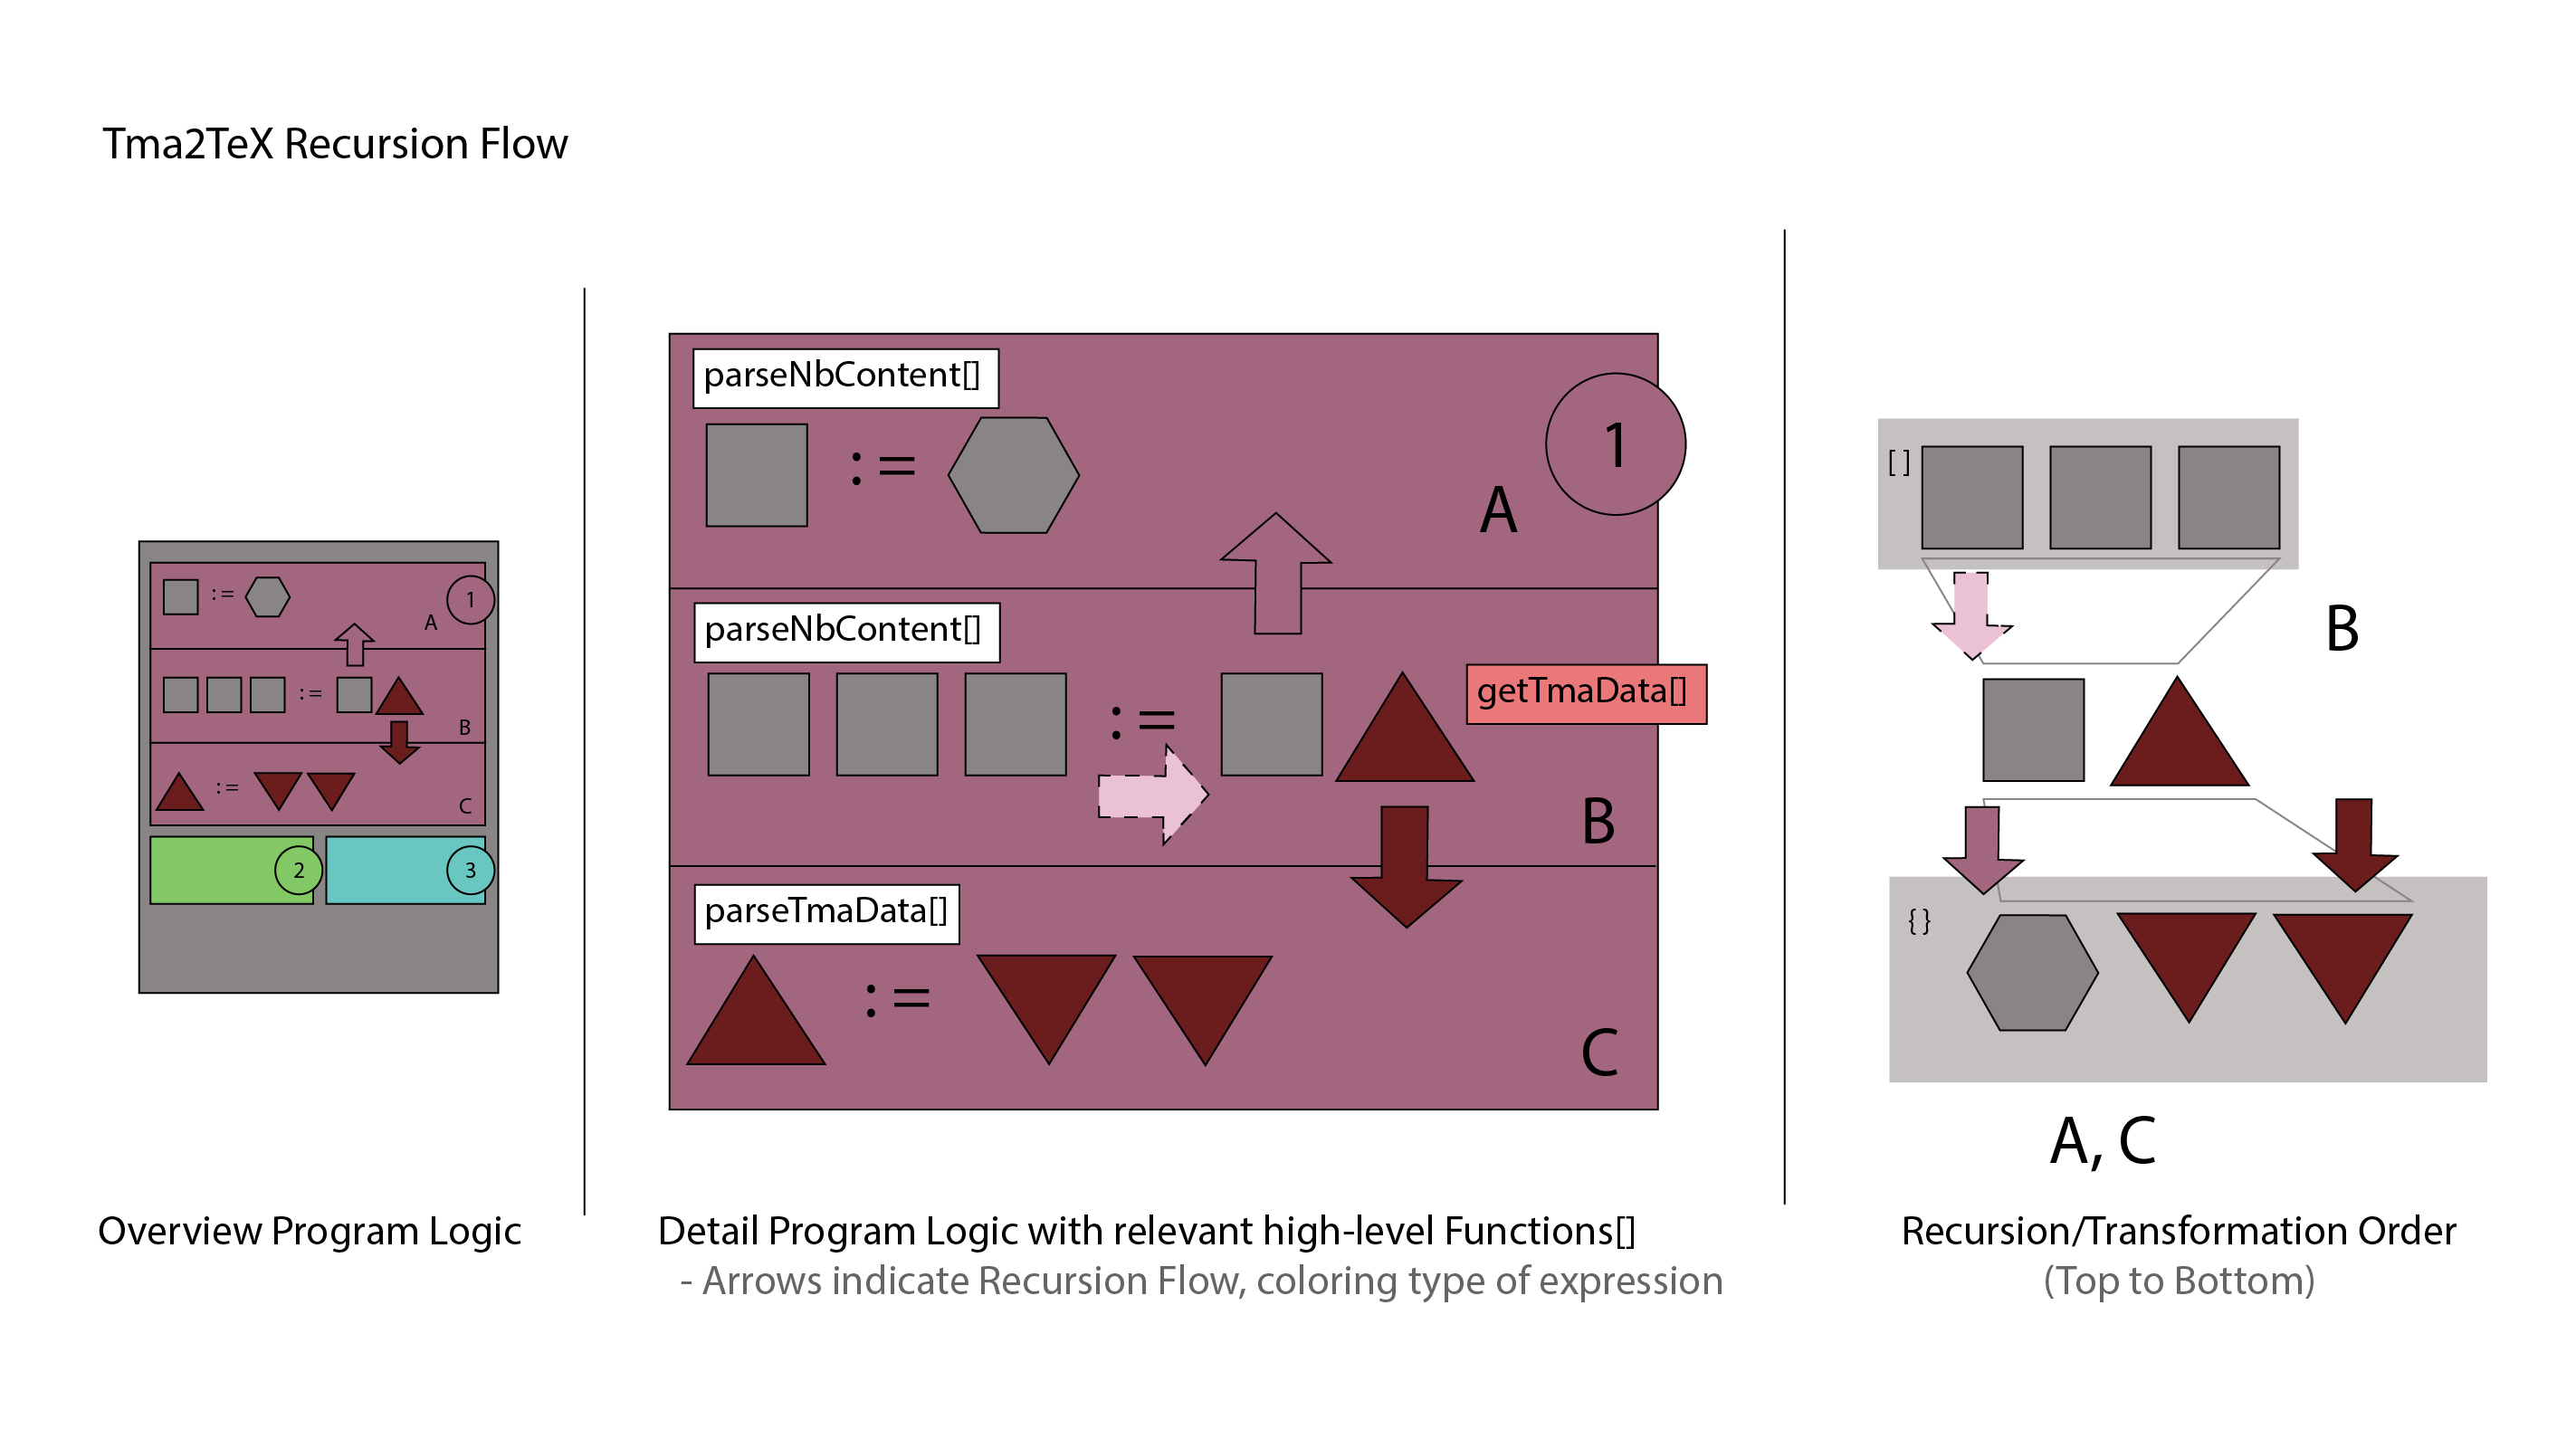
\includegraphics[scale=.35]{images/concept/Tma2Tex-Recursion-Flow-01.png}
    \caption{}
    \label{fig:high-level}
\end{figure}

Section \ref{pattern-matching-implementation} in the following chapter elaborates on the specificity rules crucial to the call order. Recursion is simple to see at this point: by adding a call to the same function on the right hand side of the rule, the rule becomes recursive. The core idea of this implementation is the fashioning of many rules that are applied according to the relevant Theorema Notebook pattern, called recursively and descended in the sense that we move from outer expression to inner-most. Indeed, we start from calling the relevant function, parseNotebookContent in the form \lstinline+parseNotebookContent[Notebook[l_List, ___]]+, that is, on the entire Notebook expression that represents a Mathematica notebook.

The same idea is applied twice, to two sets of patterns: once for general text and WL notebook expression syntax, and once for the more specific syntax specified by the Theorema Language. Hence it makes sense to speak of a double-recursion, or a double-descent, in this implementation. Theorema Language is rendered distinctively in the final \LaTeX/PDF output, to mark this distinction outwardly.

\subsection{Pattern Matching to Realize \LaTeX-Transformation of the Theorema Language Data Structure}

This subsection expands on the notion of the horizontal program dimension, after the live version of the current Theorema formula under consideration (being parsed) has been obtained, via getTmaData[]: now the goal is to generate a TeX-snippet like \verb| \IffTM{ \AndTM{ \ForallTM{ ...| with appropriate closing brackets from a formula like \verb|Theorema`Language`Iff$TM[ Theorema`Language`And$TM[ Theorema`Language`Forall$TM[ ...|. The easy suffix "TM" is chosen for the \LaTeX output, the "\$TM" visible in the Theorema Language code is the original way of keeping separate contexts. In this way Theorema may specify its own "Iff", "And", "Forall" etc., both in notebooks and the \LaTeX result of this project.

Roughly, there is a Predicate Logic distinction between operator symbols known to the language, marked by the word "Language" in the symbol name context, and knowledge outside of the language, functions and predicates with the word "Knowledge" in their context path. \cite{wolfram_research_inc_contextwolfram_2024} The parsing needs to result in square brackets for the "Knowledge"-symbols, and macro-syntax curly braces for the "Language"-symbols, with appropriate parameter placement. These macros, or commands, are then fully defined inside the \LaTeX-template file.

\section{Extensibility in Both \LaTeX and Wolfram Language}

\subsection{A Note on Evaluation Criteria and Stability}

The execution of the idea can be evaluated in terms of two core criteria. First, stability is a key criterion for this work and actually bases on generality of the patterns selected: WL and Theorema expression patters that will stand the test of time need to be selected at the development stage, and testing must include a diverse current range of Theorema notebooks. 

\subsection{WL-Messages and -Tests: Software Design Goals}

WL provides modern engineering-oriented functionality for both tests and error-handling, in the form of messages \cite{wolfram_research_inc_messagewolfram_2024} - the mechanism is part of this package such as in the case the file has not been loaded completely to provide the required formula data, see Figure \ref{fig:message-demo}.

\begin{figure}[h]
    \centering
    \includegraphics[scale=.8]{images/concept/Tma2Tex-Message-Demo.png}
    \caption{The basic idea is that every message has a definite name, of the form symbol::tag. \cite{wolfram_research_inc_textual_2024}}
    \label{fig:message-demo}
\end{figure}

Testing will make up a large part of Chapter \ref{cha:Closing}.

\subsection{Extensibility}

Extensibility at both the WL and \LaTeX levels is the other priority, with the understanding that Theorema Language might change, Wolfram Language might be updated, and additional \LaTeX commands or alternative rendering imperatives might be required.

The main extension points go as follows, where the sectioning of the code follows the final version submitted with this thesis for easier finding of the relevant code. At the WL-level:

\begin{itemize}
    \item \bold{Package Parts 1.B and 1.C}, where B covers the first recursive descent through the overall notebook structure and C the second descent into the Theorema-formula:
    
    \item \bold{formatTmaData} (1.C.3): wrapper function around the Formula-\LaTeX-output that maybe used for string replacements, for instance, at the level of the formula-\LaTeX snippets.
    \item \bold{Client-Functionality} (Part 3): both top level functions convertToLatexDoc and convertToLatexAndPdfDocs may be edited easily to suit the needs of higher-level project, while more rigid configuration details are hidden away in Part 2, especially as concerns filehandling details.
    \item \bold{Overall Package}: This project was developed as a package \"tma2tex\" but the code Parts 1 - 3 can easily be moved to another package, as long as Theorema, the overall package, is in some way available, and the global variables \lstinline+Tma2tex`\$resDir+ and \lstinline+Tma2tex`\$tmaData+ are readied.
\end{itemize}

The main extension procedure on the level of \LaTeX is to add macro-definitions in the template provided in \lstinline+Tma2tex`\$resDir+, in a file called \lstinline+tmaTemplate.tex+ in the default configuration. A sample set of macros is provided for reference in \lstinline+sampleTemplateMacros.tex+.

%\subsection{Ease of Use/Setup}
\chapter[Implementation]{Implementation, Wolfram Language Programming Paradigms and Guidelines, Integration and Deployment/Cloud}
\label{cha:Implementation}

\section{Overview of the Implementation}

The implementation followed the specification introduced in Section \ref{concept:spec}, forgoing the approach reliant on TeXForm explored at concept stage, for a simpler, direct translation mechanism, detailed in this chapter. The package specification looks like this at a high level and at the time of completing of the project:

\begin{itemize}
    \item \textbf{Package Dependencies:}
    \begin{itemize}
        \item \texttt{Theorema} 
    \end{itemize}
    
    \item (Package-public) \textbf{Global Variables/User Settings:} The dollar sign is in keeping with the Theorema (and other package) convention for global variables.
    \begin{itemize}
        \item \texttt{\$resDir}: expects a file \lstinline+tmaTemplate.tex+, and any other resources should be added here to.
        \item \texttt{\$tmaData}: set to the value of \lstinline+Theorema`Common`$tmaEnv+, callable to make background data visible to the user at any time.
    \end{itemize}

    \item \textbf{Client-Functions:} the camelcase (rathern than Pascal-case) is to distinguish the function name from WL-internal function names.
    \begin{itemize}
        \item \texttt{convertToLatexDoc}, input: a Theorema notebook/output: a .tex-file in the current directory/option: DocumentProcessingLevel goes to empty string, None or Full.
        \item \texttt{convertToLatexAndPdfDocs}: a Theorema notebook/outputs: a .tex-file and a .pdf file in the current directory/option: DocumentProcessingLevel goes to empty string, None or Full.
    \end{itemize}
\end{itemize}

\subsection{Note on Modular Programming in Wolfram Language} \label{modular-programming}

[This is related, probably: Building large software systems with Wolfram Language. See Concepts section. CompoundExpression \cite{noauthor_compoundexpressionwolfram_nodate}, Module \cite{noauthor_module_nodate}, ... Block? \cite{noauthor_blockwolfram_nodate}]

Concretely for this package, in standalone form, the package loads Theorema via a \lstinline{Needs[]} call: if the package were to be integrated to Theorema directly in future work, Theorema functionality would either be available directly or loaded in a more directed fashion in the form of relevant sub-packages.

\subsection{Overall Structure of the Package}

For organization of the code the following hierarchy and division of concerns was followed throughout, to make analysis of this academic project more structured

\begin{itemize}
    \item \textbf{Part 0: Setup} - global variables and the like.
    \begin{itemize}
        \item \texttt{Part 0.A: Public Package Variables}: \lstinline+Tma2tex\`\$resDir+, set by the user in the Package Header, and \lstinline+Tma2tex\`\$tmaData+, set to \lstinline+Theorema`Common`$tmaEnv+ initially.
        \item \texttt{Part 0.B: Private Package Variables} like \lstinline+Tma2tex`$documentProcessingLevel+ and \lstinline+tmaDataAssoc+, concerned with holding further settings and formats of the data.
    \end{itemize}
    
    \item \textbf{Part 1: Parsing with parseNbContent, getTmaData, parseTmaData}: the main recursive functionality, with the following subdivisions.   
    \begin{itemize}
        \item \texttt{Part 1.A: parseNbContent} - in this section, the concern is appropriate presentation of the output of a notebook parsing run. 
        \item \texttt{Part 1.B: parseNbContent at higher level}, concerned with bridging to the Theorema Language.
        \item \texttt{Part 1.C: getTmaData/parseTmaData}, concerned with processing the Theorema Language.
    \end{itemize}
    
    \item \textbf{Part 2: Filehandling}
    \begin{itemize}
        
    \end{itemize}

    \item \textbf{Part 3: Client Functions}
    \begin{itemize}
        
    \end{itemize}
\end{itemize}

\section{High Level Programming in Practice}

In high-level programming within WL, the focus is primarily on manipulating symbolic expressions and applying transformation rules rather than managing low-level implementation details. This abstraction layer allows developers to craft powerful programs with minimal code, leveraging the language's built-in functions for data manipulation, pattern matching, and rule-based transformations. [Ref.]

The Wolfram Language offers several key features that support high-level programming, as seen in both filehandling and the client functions in this project:

\begin{itemize}
    \item \textbf{Symbolic Computation:} All expressions in the Wolfram Language are treated symbolically, allowing functions to operate on concrete data, as well as symbolic representations of mathematical expressions, code, or documents.
    
    \item \textbf{Pattern Matching and Transformation Rules:} Advanced pattern matching capabilities facilitate the definition of rules for transforming expressions, simplifying the implementation of complex algorithms in a clear and concise manner.
    
    \item \textbf{Functional Programming Constructs:} Functions such as \texttt{Map}, \texttt{Apply}, and \texttt{Fold} support a functional programming style, enabling operations on lists and other data structures without explicit loops.
    
    \item \textbf{Built-In Algorithms and Computational Knowledge:} The language integrates a vast repository of algorithms for numerical computation, algebra, statistics, and other domains, alongside access to curated data, allowing for the resolution of problems at a high level without the need to develop standard methods from scratch.
    
    \item \textbf{Notebook Interface:} The Wolfram Language is often used within interactive notebooks, providing a rich environment for computation, visualization, and dynamic document creation. This interface enhances the development process by offering immediate feedback and facilitating exploratory programming.
\end{itemize}

[Ref.]

By leveraging these features, developers can write programs that are not only more concise and readable but also easier to maintain and adapt, emphasizing the core logic of their applications rather than low-level programming concerns.

\subsection{Client Functions}

The main client function in this package, relying heavily on high level programming, is \texttt{convertToLatexDoc}. This function is responsible for converting a given Theorema notebook to a LaTeX document. The function takes a notebook path and optional settings for the document processing level. It retrieves the notebook content, parses it, and fills a LaTeX template with the extracted data such as the title, author, and date. The function then exports the filled content to a \texttt{.tex} file. 

This function is also called by \texttt{convertToLatexAndPdfDocs}, which extends its functionality by converting the LaTeX file to a PDF. After calling \texttt{convertToLatexDoc}, it checks for successful conversion and then uses the \texttt{pdflatex} command to compile the LaTeX file into a PDF document.

These two functions, \texttt{convertToLatexDoc} and \texttt{convertToLatexAndPdfDocs}, are the core client functions intended to be called by Theorema, the user. They encapsulate the primary operations necessary for converting Theorema notebooks into LaTeX and PDF documents, providing a seamless integration with the Theorema environment for document processing.

\begin{verbatim}
Options[convertToLatexDoc] = {DocumentProcessingLevel -> ""};
convertToLatexDoc[notebookPath_, OptionsPattern[]] := Module[{nb, content, 
    latexPath, latexTemplatePath, resourceDir = $resDir, texResult, sownData, 
    filledContent, closeFlag = False, documentProcessingLevel},
  If[Length[$tmaData] == 0, 
    Message[tmaDataImport::empty, "The Theorema-Formula-Datastructure is empty. 
    Did you evaluate a Theorema notebook before loading the package and calling 
        the conversion function?"];
    Return[$Failed]
  ];

  documentProcessingLevel = OptionValue[DocumentProcessingLevel];
  If[documentContentProcessingLevel =!= "", 
    SetDocumentProcessingLevel[documentProcessingLevel]
  ];

  nb = If[isNotebookOpen[notebookPath],
    NotebookOpen[notebookPath],
    NotebookOpen[notebookPath, Visible->False]; closeFlag = True];
  
  content = NotebookGet[nb];
  NotebookEvaluate[content];
  latexPath = getLatexPath[notebookPath];
  latexTemplatePath = getLatexTemplatePath[notebookPath]; 

  {texResult, sownData} = Reap[parseNbContent[content], {"title", "author", "date"}];
  filledContent = fillLatexTemplate[resourceDir,
    <|
      "nbContent" -> texResult,
      "nbTitle" -> First[sownData[[1, 1]]],
      "nbAuthor" -> First[sownData[[2, 1]]],
      "nbDate" -> First[sownData[[3, 1]]]
    |>];
  Export[latexPath, filledContent, "Text"];
  If[closeFlag === True, NotebookClose[notebookPath]]; 
]

Options[convertToLatexAndPdfDocs] = {DocumentProcessingLevel -> ""};
convertToLatexAndPdfDocs[notebookPath_, OptionsPattern[]] := Module[{latexPath, 
    pdfPath, compileCmd, conversionResult},
  conversionResult = convertToLatexDoc[notebookPath, 
    DocumentProcessingLevel->OptionValue[DocumentProcessingLevel]];
  If[conversionResult === $Failed,
    Return[$Failed]
  ];
  latexPath = getLatexPath[notebookPath];
  pdfPath = StringReplace[latexPath, ".tex" -> ".pdf"];
  compileCmd = 
   "pdflatex -interaction=nonstopmode -output-directory=" <> 
    DirectoryName[latexPath] <> " " <> latexPath;
  RunProcess[{"cmd", "/c", compileCmd}];
]
\end{verbatim}

\subsection{File-handling and \LaTeX Details}

\paragraph{Key Functionalities:}

The primary functionalities of the file-handling code can be summarized as follows:

\begin{itemize}
    \item \textbf{Writing to LaTeX Files:} The function \texttt{writeToLatexDoc} is responsible for writing the parsed content of a Theorema notebook to a new LaTeX file. This function opens a file stream using the provided path (\texttt{latexPath}), writes the parsed content (\texttt{nbContent}) to it, and then closes the stream. This process ensures that the data is efficiently transferred from the internal representation to a format suitable for LaTeX processing.

    \item \textbf{Generating LaTeX File Paths:} The function \texttt{getLatexPath} constructs the full path for the new LaTeX file by appending the \texttt{.tex} extension to the base name of the original Theorema notebook file. This method ensures that the LaTeX file is stored in the same directory as the source notebook, maintaining a logical and consistent file organization.

    \item \textbf{Locating LaTeX Templates:} The function \texttt{getLatexTemplatePath} similarly constructs the path for a LaTeX template file. This template file serves as a wrapper or framework for the main content LaTeX file, ensuring proper formatting and structure in the final output.

    \item \textbf{Filling the LaTeX Template:} The function \texttt{fillLatexTemplate} handles the process of importing a predefined LaTeX template (\texttt{tmaTemplate.tex}) from the specified directory and dynamically filling it with content from an association (\texttt{data}). This template-based approach allows for the flexible customization of the LaTeX document according to different requirements or styles.
\end{itemize}

\paragraph{Directory Structure and File Organization:}

The implementation works with a well-defined directory structure where the following components are needed:

\begin{itemize}
    \item \textbf{Notebook Directory:} The primary directory where the original Theorema notebook files are located. The LaTeX files generated by \texttt{getLatexPath} and \texttt{getLatexTemplatePath} are stored in the same directory, preserving the association between the source notebooks and their corresponding LaTeX outputs.

    \item \textbf{Template Directory:} A subdirectory containing the LaTeX template file (\texttt{tmaTemplate.tex}). This template is imported by the \texttt{fillLatexTemplate} function and filled with content to create a complete LaTeX document. The template file is assumed to be reusable across multiple notebook conversions, providing a consistent document structure.

    \item \textbf{Resulting Files:} The resulting files from this process include:
    \begin{itemize}
        \item A LaTeX content file named according to the original notebook (\texttt{.tex} extension).
        \item The final PDF document generated from the filled LaTeX template, if calling the appropriate client function.
    \end{itemize}
\end{itemize}

\section{Implementation of (Double) Recursive Descent with Pattern Matching} \label{pattern-matching-implementation}

\subsection{General Remarks on Pattern Matching, and Execution Order, in Wolfram Language}

There are various nuances when it comes to pattern matching in Wolfram Language. One example is this rendering of a "DisplayFormula," that is, a formula written closely to frontend rendering (box structure first, rather than formula first), without Wolfram or Theorema Language logic in mind.

Notebook WL code is given by the following code snippet, illustrating the front-end-orientation of the code.

\begin{verbatim}
{Cell[BoxData[
 FormBox[
  RowBox[{
   RowBox[{"(", 
    RowBox[{
     UnderscriptBox["\\[ForAll]", "x"], 
     RowBox[{"(", 
      RowBox[{
       RowBox[{"P", "[", "x", "]"}], "\\[Or]", 
       RowBox[{"Q", "[", "x", "]"}]}], ")"}]}], ")"}], "\\[And]", 
   ... }]}, 
  TraditionalForm]], "DisplayFormula", ...
 CellID->2121253064,ExpressionUUID->"384e1c8f-1530-48b6-9503-bea644c47327"],
 ...}
\end{verbatim}

The functions BoxData, FormBox, RowBox and UnderscriptBox take care of minimal formatting required for a readable rendering. 

These expressions can be parsed recursively with the following WL code to test execution order.

\begin{verbatim}
parseNbContent[l_List] := If[$documentProcessingLevel == "Full", 
    "\\colordiamond{blue}", ""]
parseNbContent[l_List] /; MemberQ[l, _Cell] := 
    StringJoin[If[$documentProcessingLevel == "Full", 
        "\\colordiamond{purple}", ""], ToString /@ parseNbContent /@ l] 
...
parseNbContent[Cell[BoxData[FormBox[content_, 
    TraditionalForm]], "DisplayFormula", ___]] := 
        If[$documentProcessingLevel != "None", StringJoin["\\begin{center}", 
            parseNbContent[content], "\\end{center}\n"], ""]
\end{verbatim}

While the latter pattern is highly specific, there is only a small difference (involving a condition) between the first two rules, concerned with parsing lists, like the one in the previous example, marked by curly braces.

When multiple rules are applicable to a given expression, WL uses specificity to determine which rule to apply. The specificity rule in pattern matching operates on the principle that more specific patterns are chosen over more general ones when multiple patterns match an expression. Here's how specificity is determined in WL:

\begin{itemize}
    \item Literal Patterns Over Pattern Objects: A pattern that exactly matches an expression is considered more specific than a pattern involving pattern objects (like \lstinline+_+, \lstinline+__+, \lstinline+___+, or named patterns using \lstinline+_type+, etc.). For example, a rule for \lstinline+f[1]+ is more specific than a rule for \lstinline+f[x_].
    \item Constrained Patterns Over Unconstrained: Patterns with conditions (\lstinline+/;+) or pattern tests are more specific than those without. For example, \lstinline+f[x_ /; x > 0]+ is more specific than \lstinline+f[x_]+.
    \item Constrained Patterns Over Unconstrained: Patterns with conditions (\lstinline+/;+) or pattern tests are more specific than those without. For example, \lstinline+f[x_ /; x > 0]+ is more specific than \lstinline+f[x_]+.
    \item Length and Structure: Patterns that match expressions with more specific structure or length are preferred. For example, \lstinline+f[{x_, y_}]+ is more specific than \lstinline+f[_List]+, and \lstinline+f[x_, y_]+ is more specific than \lstinline+f[___]+.
    \item Head Specificity: Patterns specifying a head are more specific than patterns without a head specification. For example, \lstinline+f[x_Integer]+ is more specific than \lstinline+f[x_]+.
    \item Order of Definition: When patterns have the same specificity, the rule that was defined first is chosen. This is relevant for user-defined rules where the specificity might appear equal.
    \item Nested Patterns: In nested patterns, specificity is considered at each level of nesting. A pattern that is more specific at any level of nesting is considered more specific overall.
\end{itemize}

[Ref.]

\subsection{Limited Approach of Specific Pattern Matching Rules}

Part 1.A in the code defines patterns as basic cell structures to extract certain information, as in this case:

\begin{verbatim}
(* -- Part 1.A.1 -- Text Expressions (at the Cell Level): 
    Not processed if DocumentProcessingLevel = "None", otherwise yes. *)
parseNbContent[Cell[text_String, "Text", ___]] := 
    If[$documentProcessingLevel != "None", "\\begingroup \\section*{} " 
        <> text <> "\\endgroup \n\n", ""]
parseNbContent[Cell[text_String, "Section", ___]] := 
    If[$documentProcessingLevel != "None", "\\section{" 
        <> text <> "}\n\n", ""]
\end{verbatim}

There are also rules for front-end displayed formulas used in the main text, to display the main content relevant for the reader:

\begin{verbatim}
parseNbContent[UnderscriptBox["\[Exists]", cond_]] :=
    If[$documentProcessingLevel != "None", 
    "\\underset{" <> parseNbContent[cond] <> "}{\\exists}", ""]
parseNbContent[UnderscriptBox["\[ForAll]", cond_]] :=
    If[$documentProcessingLevel != "None", 
    "\\underset{" <> parseNbContent[cond] <> "}{\\forall}", ""]
\end{verbatim}

To accomplish coherent recursive pattern matching as it is initiated in the preceeding example, the patterns need to be defined down to the symbol level.

\begin{verbatim}
parseNbContent[RowBox[{left_, "\[And]", right_}]] := 
    If[$documentProcessingLevel != "None", StringJoin[parseNbContent[left], 
    " \\land ", parseNbContent[right]], ""]
parseNbContent[RowBox[{left_, "\[Or]", right_}]] := 
    If[$documentProcessingLevel != "None", StringJoin[parseNbContent[left], 
    " \\lor ", parseNbContent[right]], ""]
parseNbContent[RowBox[{left_, "\[DoubleLeftRightArrow]", right_}]] := 
    If[$documentProcessingLevel != "None", StringJoin[parseNbContent[left], 
    " \\Leftrightarrow ", parseNbContent[right]], ""]
\end{verbatim}

The approach is naturally limited: foreseeing every possible symbol used in mathematics, even a subset, requires an extensive set of rules, the like is implemented under the hood in the TeXForm, as is explored in the chapter on the concept: this approach is only implemented so far, instead making use of \lstinline+parseNbContent[]+ to essentially locate the major features like titles and sections in the Theorema notebook, and find the appropriate jumping off point (for parsing) into the Theorema formula.

This happens in Part 1.B: the pattern

\begin{verbatim}
    Cell[CellGroupData[{Cell[headertext_, "EnvironmentHeader", headeroptions___], 
                        Cell[formulaboxdata_, "FormalTextInputFormula", options___], 
                        furtherNotebookEnvCells___}, 
                       envOptions___]]
\end{verbatim}

is captured and one line in the relevant function call reads:

\begin{verbatim}
    formatTmaData@parseTmaData[getTmaData[cellID]]
\end{verbatim}

The \lstinline+cellID+, extracted from the \lstinline+options+ in the preceeding pattern, is used to \lstinline+getTmaData+ from the environment variable: now this is parsed in a second recursive descent (with a slightly different approach), and finally formatted as needed on string- rather than expression-level.

\subsection{Generalized Parsing Approach for Theorema Data}

\paragraph{Core Parsing Function:}

The function \texttt{parseTmaData} uses pattern matching to handle various types of expressions. The first definition, 

\begin{verbatim}
parseTmaData[op\_?isTmaLanguageSymbol[args\_\_\_]] := 
  Module[{nextOp, argList, parsedArgs}, 
  nextOp = prepareSymbolName[op]; 
  argList = {args}; 
  parsedArgs = Switch[
    Length[argList], 
    1, "{" <> parseTmaData[argList[[1]]] <> "}", 
    2, "{" <> parseTmaData[argList[[1]]] <> "}
        {" <> parseTmaData[argList[[2]]] <> "}", 
    3, "{" <> parseTmaData[argList[[1]]] <> "}
        {" <> parseTmaData[argList[[3]]] <> "}", 
    _, ""
  ]; 
  " \\" <> ToString[nextOp] <> parsedArgs
  ]
\end{verbatim}

handles expressions where the operator is recognized as a language symbol using the predicate \texttt{isTmaLanguageSymbol}. The function utilizes a \texttt{Module} to locally define variables and processes the arguments using a \texttt{Switch} statement, which handles different numbers of arguments. The main thing here: this covers the Theorema Language case of an epxression that needs to be converted to something like

\begin{verbatim}
    \RNGTM{ \SIMPRNGTM{ \VARTM{a}}}
\end{verbatim}

for example: The ranges and variable expressions are transformed to parameterizable \LaTeX macros that can be defined exactly the way the user wishes, \LaTeX-side: it is a generalized approach.

\paragraph{Alternative Parsing Cases:}

Several alternative cases are defined to handle different types of expressions:

\begin{itemize}
    \item \textbf{Non-Language Operators:} The second alternative matches expressions where the operator is not a recognized language symbol:

    \begin{verbatim}
    parseTmaData[op\_[args\_\_\_]] := 
      Module[{nextOp, argList, parsedArgs}, 
      nextOp = prepareSymbolName[op]; 
      argList = {args}; 
      parsedArgs = Switch[
        Length[argList], 
        1, "[" <> parseTmaData[argList[[1]]] <> "]", 
        2, "[" <> parseTmaData[argList[[1]]] <> ", " 
            <> parseTmaData[argList[[2]]] <> "]", 
        _, ""
      ]; 
      " " <> ToString[nextOp] <> parsedArgs
      ]
    \end{verbatim}

    This alternative similarly handles the parsing, but formats the output using square brackets instead of curly braces, reflecting a different LaTeX macro style reserved for predicate expressions like \lstinline+P[x]+, for example. This is considered Theorema Knowledge and marked as such in the typical context paths found in Theorema language expressions.

    \item \textbf{Special Two-Argument Sets:} Another special case handles expressions where two sets of arguments are present:

    \begin{verbatim}
    parseTmaData[op\_?isTmaLanguageSymbol[args\_\_\_][args2\_\_\_]] := 
      Module[{nextOp, argList, argList2, parsedArgs, parsedArgs2}, 
      nextOp = prepareSymbolName[op]; 
      argList = {args}; 
      parsedArgs = Switch[...];
      argList2 = {args2}; 
      parsedArgs2 = Switch[...]; 
        " \\" <> ToString[nextOp] <> parsedArgs <> parsedArgs2
      ]
    \end{verbatim}

    Here, the function handles two levels of arguments, which are independently parsed and concatenated.

    \item \textbf{Literal Numbers and Terminal Expressions:} Additional cases handle literal integers and terminal expressions that do not require further parsing:

    \begin{verbatim}
    parseTmaData[i\_Integer] := ToString[i]

    parseTmaData[ax\_] := prepareSymbolName[ax]
    \end{verbatim}

    These cases ensure that numbers and final symbolic expressions are converted directly to their string representations or appropriately prepared names.

\end{itemize}

\paragraph{Auxiliary Functions:}

Two auxiliary functions, \texttt{isTmaLanguageSymbol} and \texttt{prepareSymbolName}, are defined to assist with parsing:

\begin{verbatim}
isTmaLanguageSymbol[f\_Symbol] := 
    With[{n = SymbolName[f], c = Context[f]}, c === "Theorema`Language`"]
isTmaLanguageSymbol[f\_] := False
\end{verbatim}

The function \texttt{isTmaLanguageSymbol} determines whether a given symbol belongs to the \texttt{Theorema`Language`} context. 

\begin{verbatim}
prepareSymbolName[op\_Symbol] := 
    With[{n = SymbolName[op]}, 
    If[StringTake[n, -3] == "$TM", 
        If[StringTake[n, 4] == "VAR$", StringDrop[StringDrop[n, 4], -3], 
            If[isTmaLanguageSymbol[op], StringDrop[n, -3] <> "TM", StringDrop[n, -3]], 
        If[StringTake[n, -1] == "$", StringDrop[n, -1] <> "TM", n <> "TM"]]
    ]
\end{verbatim}

The \texttt{prepareSymbolName} function is responsible for converting Theorema symbols into valid LaTeX macro names, ensuring that symbols conform to the required formatting conventions for their respective contexts.


\chapter{Closing Remarks}
\label{cha:Closing}

%%%-----------------------------------------------------------------------------
\appendix                                                             % Appendix 
%%%-----------------------------------------------------------------------------

\chapter{Technical Documentation/Source Code}
\label{app:Source}

% Soure Code provision method

The project repository is synced in its entirety with this document and listed below. 

Development in the main branch is frozen on the submission date. Any changes after the submission of this document will be separated into a new branch. The final version will also be submitted with this document, see Appendix B (Supplementary Materials).

% Online Repo (for access after print)

The final version with any further development can be viewed online at \url{https://github.com/heseltime/Tma2TeX}.

% Source Code includes, GitHub Synch (Overleaf Premium Feature, up to print)

\lstinputlisting[language=Mathematica, caption=Wolfram Language example]{test.m} % Technical Documentation/Source Code
\chapter{Supplementary Materials}
\label{app:Supplement}


List of supplementary data submitted to the degree-granting institution for archival storage
(in ZIP format).

% Use this as an example only, adapt the structure to your requirements!

\section{PDF Files}
\begin{FileList}{/}
\fitem{thesis.pdf} Bachelor thesis (complete document)
\end{FileList}

\section{Program Files}
\begin{FileList}{/media}
\fitem{*.wl, *.m} TODO
\end{FileList}




 % Contents of any submitted project archive
\chapter{Sample Document FirstTour}
\label{app:Sample}

% Soure Code provision method

The main sample document this project is tested with is included in its final LaTeX-transformed and PDF-rendered output format: the .tex-file this document is rendered from is printed in Appendix A and the original Wolfram Language notebook is included in the submission (and online) repository detailed in Appendix B.

% Sample Document to include with thesis

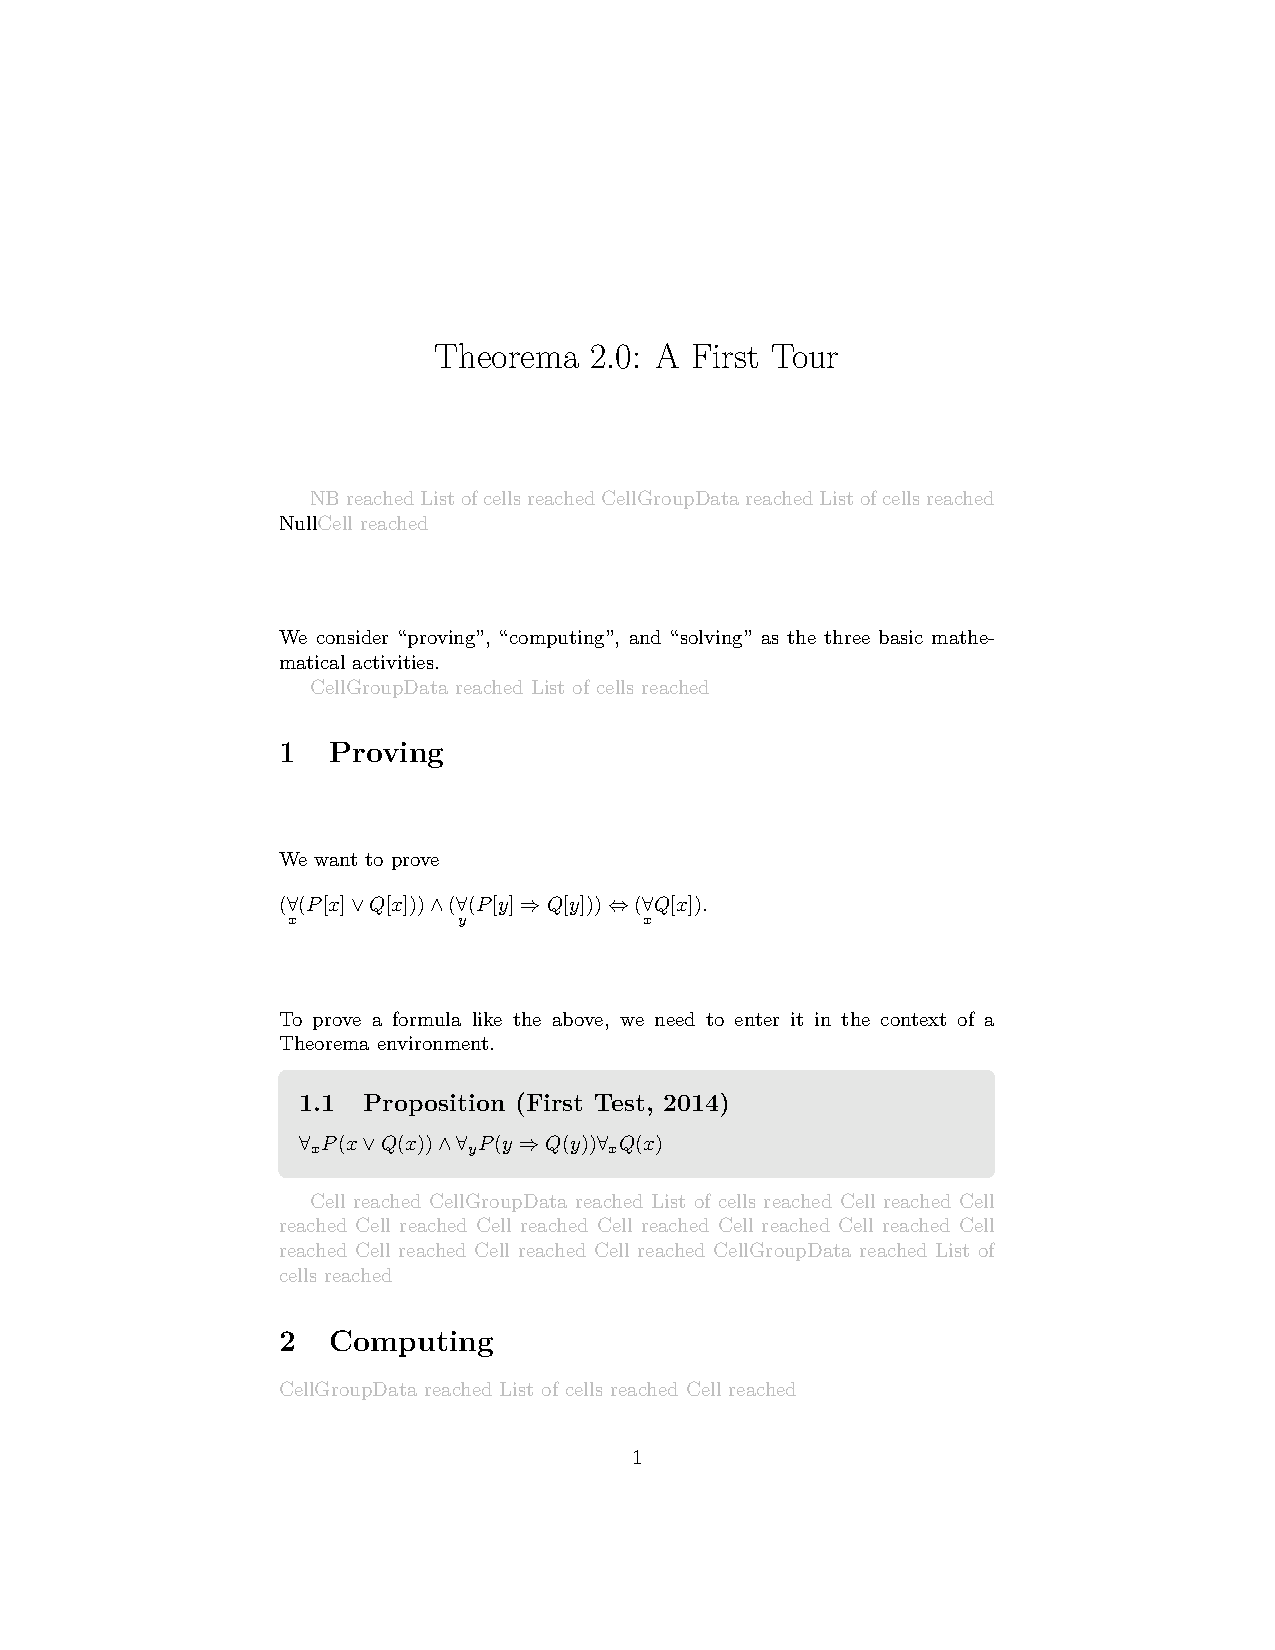
\includepdf[pages=-,frame,scale=0.8,pagecommand={}]{tma2tex/FirstTour.pdf} % Contents of any submitted project archive
\chapter{Exposé: A Tree Pattern Function in Mathematica}
\label{app:Expose}

% Soure Code provision method

An exposé of the programming paradigms highlighted in Chapter \ref{cha:Theory} is included with this thesis work: It was produced as part of the companion seminar class, "Wissenschaftliches Arbeiten," i.e. Scientific Research and Writing, and serves to deliver some additional Theory about programming in WL, separately from the project focus of the main work. The author hopes this aids the interested reader and would like to point out that the document is interesting formally in that it was produced inside a Mathematica notebook, so that the cells containing text and executable WL code are of equal order inside an overall WL notebook expression, as outlined in \ref{cha:Introduction}, concerning WL expressions as document representation: as opposed to this project's \LaTeX transformation, or the native transformation also referenced in \ref{cha:Introduction}, this format represents another way, the non-\LaTeX, Mathematica-native PDF-export, for making available WL notebook content.

% Sample Document to include with thesis

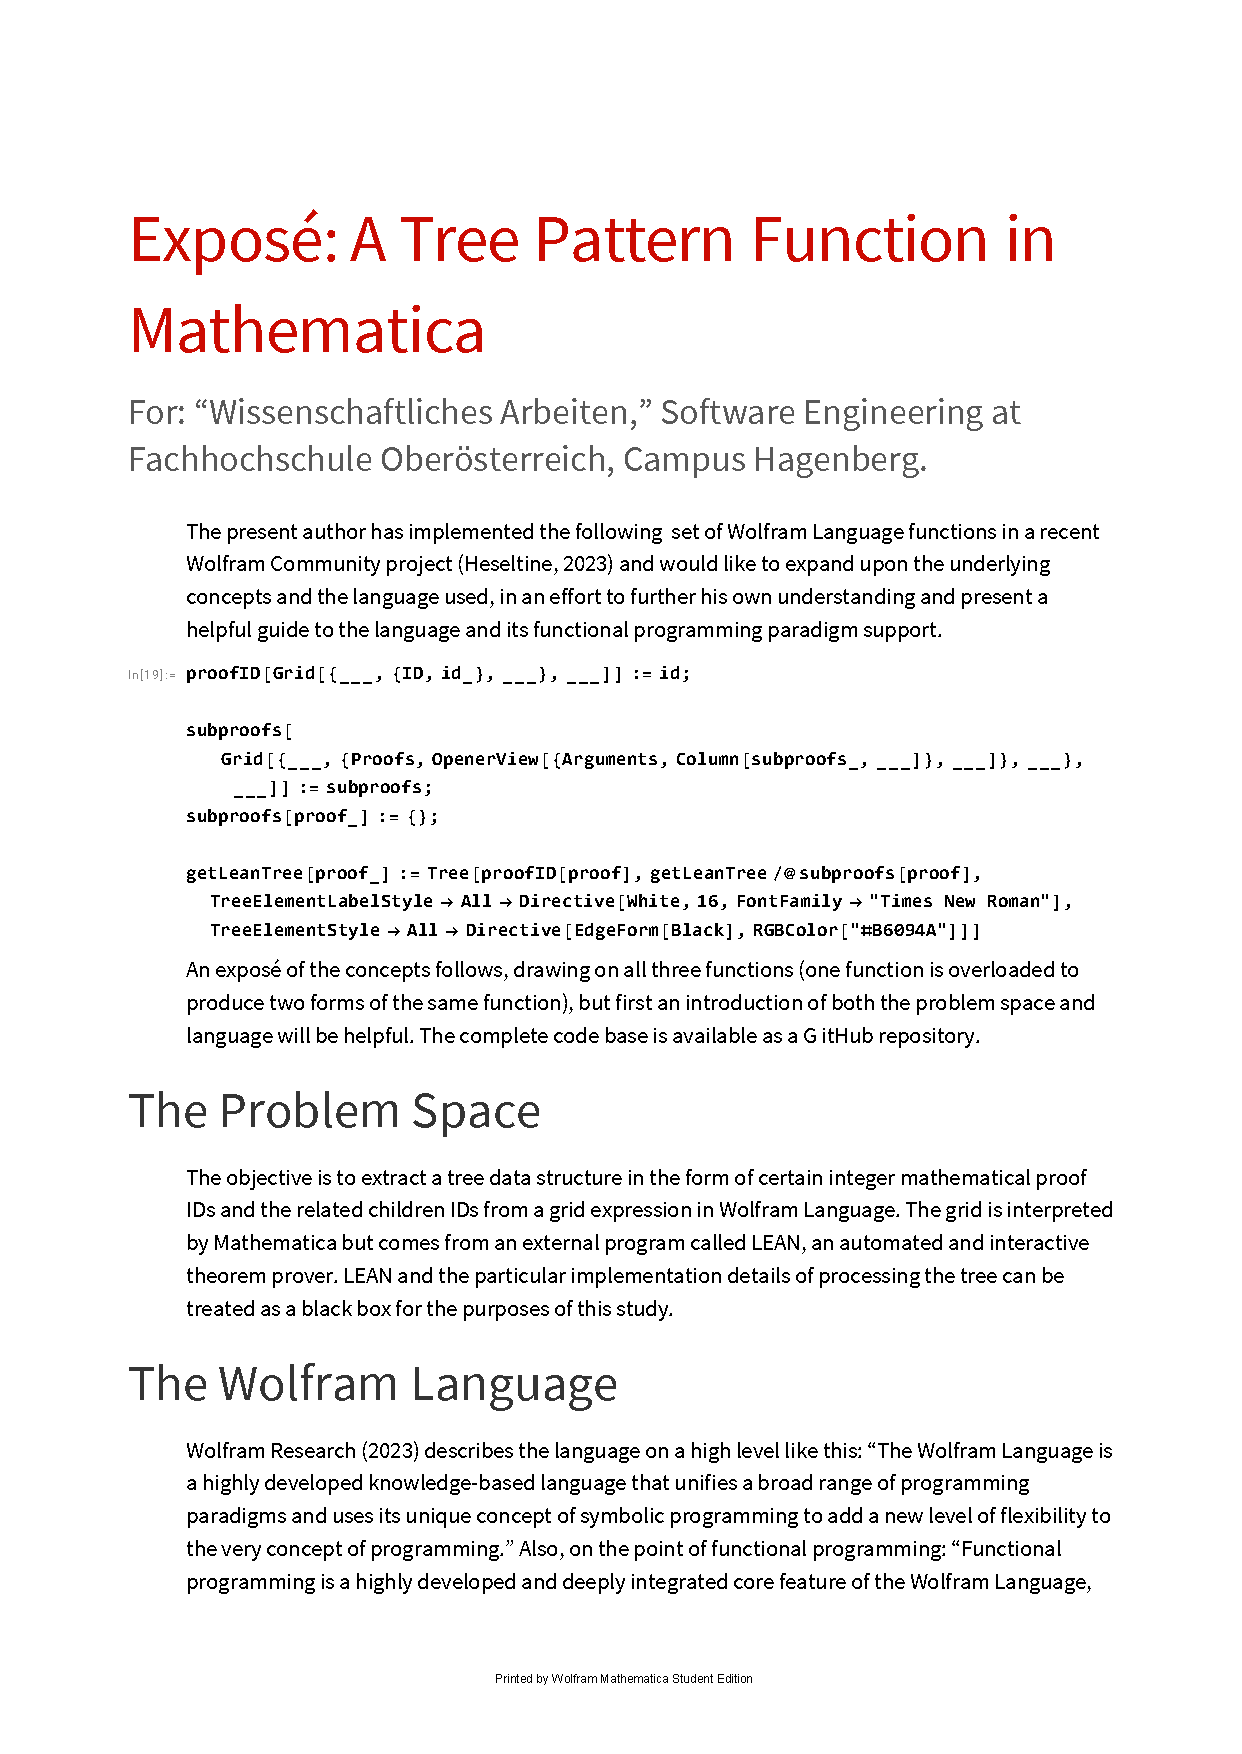
\includepdf[pages=-,frame,scale=0.95,pagecommand={}]{furtherpdfincludes/expose-tree-pattern-function-native-export.pdf} % Contents of any submitted project archive

%%%-----------------------------------------------------------------------------
\backmatter                           % Back part (bibliography, glossary, etc.)
%%%-----------------------------------------------------------------------------

\MakeBibliography % References

%%%-----------------------------------------------------------------------------
% Special page for checking print https://www.overleaf.com/project/6529637a00e0d9663e2ef77csizehttps://www.overleaf.com/project/6529637a00e0d9663e2ef77c
%%%-----------------------------------------------------------------------------

\chapter*{Check Final Print Size}

\begin{center}
{\Large --- Check final print size! ---}

\bigskip

\calibrationbox{100}{50} % width/height of box in mm

\bigskip

{\Large --- Remove this page after printing! ---}

\end{center}



%%%-----------------------------------------------------------------------------
\end{document}
%%%-----------------------------------------------------------------------------
